\documentclass[a0paper,portrait]{baposter}
\usepackage[french]{babel}


\usepackage{wrapfig}
\usepackage{lmodern}
\usepackage{lipsum,graphicx}
\usepackage{fontspec}
\usepackage{advdate}
\usepackage{svg}
\usepackage{xcolor}
\usepackage{tabularx}


% Set main font (Abraham)
%\setmainfont[
%    Path = font/Abraham/,
%    Extension = .otf,
%    % SmallCapsFont = *-smallcaps,
%    BoldFont = *-bold, % Outline
%    ItalicFont = *-italic, % Italic
%    BoldItalicFont = *-bolditalic % Outline Italic
%]{abraham}

%

\graphicspath{{figures/}} % Directory in which figures are stored

\newcommand{\compresslist}{%
\setlength{\itemsep}{0pt}%
\setlength{\parskip}{1pt}%
\setlength{\parsep}{0pt}%
}

\newenvironment{boenumerate}
  {\begin{enumerate}\renewcommand\labelenumi{\textbf\theenumi.}}
  {\end{enumerate}}


\begin{document}

\definecolor{Mycolor1}{HTML}{3FFF00}
\definecolor{Mycolor2}{HTML}{0FF000} %0FF000

\begin{poster}
{
grid=false,
headerborder=open, % Adds a border around the header of content boxes
colspacing=1em, % Column spacing
bgColorOne=white, % Background color for the gradient on the left side of the poster
bgColorTwo=white, % Background color for the gradient on the right side of the poster
borderColor=Mycolor1, % Border color
headerColorOne=Mycolor2, % Background color for the header in the content boxes (left side)
headerColorTwo=Mycolor2, % Background color for the header in the content boxes (right side)
headerFontColor=white, % Text color for the header text in the content boxes
boxColorOne=white, % Background color of the content boxes
textborder=rounded, %rectangle, % Format of the border around content boxes, can be: none, bars, coils, triangles, rectangle, rounded, roundedsmall, roundedright or faded
eyecatcher=false, % Set to false for ignoring the left logo in the title and move the title left
headerheight=0.08\textheight, % Height of the header
headershape=rounded, % Specify the rounded corner in the content box headers, can be: rectangle, small-rounded, roundedright, roundedleft or rounded
headershade=plain,
headerfont=\Large\textsf, % Large, bold and sans serif font in the headers of content boxes
%textfont={\setlength{\parindent}{1.5em}}, % Uncomment for paragraph indentation
linewidth=1pt % Width of the border lines around content boxes
}
{}
%
%----------------------------------------------------------------------------------------
%	TITLE AND AUTHOR NAME
%----------------------------------------------------------------------------------------
%
{\textsf{{Tableau de bord - Éco-Marathon Shell 2023}}} % Titre en Sans Serif
{\sf\vspace{0.1em}\\
Mécanique  -  {\AdvanceDate[0]\today} 
\vspace{0.1em}\\
\small{ Période couverte du {\AdvanceDate[-7]\today} au {\AdvanceDate[0]\today}
}
}
{
\includegraphics[width=.1\linewidth]{img/udes.png}} % TU Dublin logo


% this states the box starts at column 0 (edge of page), row 0 (top of page) for a span of 3 (columns wide)
\headerbox{Objectif de projet}{name=objectif,column=0,row=0, span=3}{
Créer un véhicule efficace à propulsion électrique pour participer et gagner la compétition Shell-éco marathon dans la division ''véhicule urbain'' en 2023

\foo 
\begin{flushleft}
    \bf
QUOTE de la semaine : Never give up until youve given out all your very best. It’s better to fail trying, than wondering what could have happened if you tried.
\end{flushleft}
\vspace{2cm} %remove this, only added for spacing

}

% this states the box starts at column 0 (edge of page), directly below the box labelled introduction for a span of 1 (column wide)
\headerbox{Objectifs de session}{name=objectif_session,column=1,below=objectif,span=2}{

%\vspace{0.15cm}
\centering
{\begin{tabularx}{\linewidth}{
    >{\hsize=1.0\hsize}X
    >{\hsize=0.5\hsize}X
    >{\hsize=1.0\hsize}X
    >{\hsize=0.5\hsize}X
  }
    
    \textbf{Objectif} & \textbf{Système} & & \textbf{Avancement} \\
     Terminer la modélisation de sous-systèmes & Simulateur &  & 95\% \\
     Conception et fabrication du système d'attaches avant & Suspension &  & 85\% \\
     Conception détaillée Ackermann et fit & Direction &  & 70\% \\
     Conception détaillée du ch\^assis & ch\^assis & & 65\% \\
     Conception détaillée et commandes de composantes & Freins &  &  60\% 
     \\
      Conception détaillée de la coque & Coque && 50\% 
      \\
       
  \end{tabularx}
    
    
 % Template des Objectifs rencontés:
 %
 % Objectif : l'objectif de la session
 % Système  : le nom ou numéro système que l'objectif touche ex: Simulateur ou SIM1
 % &  & = ESPACE POUR LE FORMATAGE NE PAS ENLEVER
 % Avancement : Pourcentage estimé d'avancement de l'objectif.
 %
 %  
 %  \textbf{Objectif} & \textbf{Système} &  & \textbf{Avancement}\\
 %   Objectif & Système &  & Avancement \\
 %   Objectif & Système &  & Avancement \\
 %   Objectif & Système &  & Avancement \\
 %   Objectif & Système &  & Avancement \\
 %   Objectif & Système &  & Avancement \\





}

%\vspace{0.2cm} % spacing vertical

}

% this states the box starts at column 0 (edge of page), directly below the box labelled subtopic1 for a span of 1 (column wide)
\headerbox{Ordre du jour}{name=ordre_jour,column=0,below=objectif,span=1}{

\begin{itemize}
    \item \textbf{Rencontre gestion :}
    \begin{enumerate}
        \item Projet ordre tableau de bord fini
        \item Starr ccm+ fonctionne
        \item site web en cours
    \end{enumerate}
    \item \textbf{Rencontre technique :}
    \begin{enumerate}
        \item 
        \item 
    \end{enumerate}
\end{itemize}

\vspace{0.05cm} % spacing vertical
}

\headerbox{Membres}{name=membres,column=2,below=ordre_jour,span=1}{
\vspace{0.3cm}


% inserts an image inside the box, 5 rows high | r = on the right along side text 
\begin{wrapfigure}[5]{r}{0.25\textwidth}
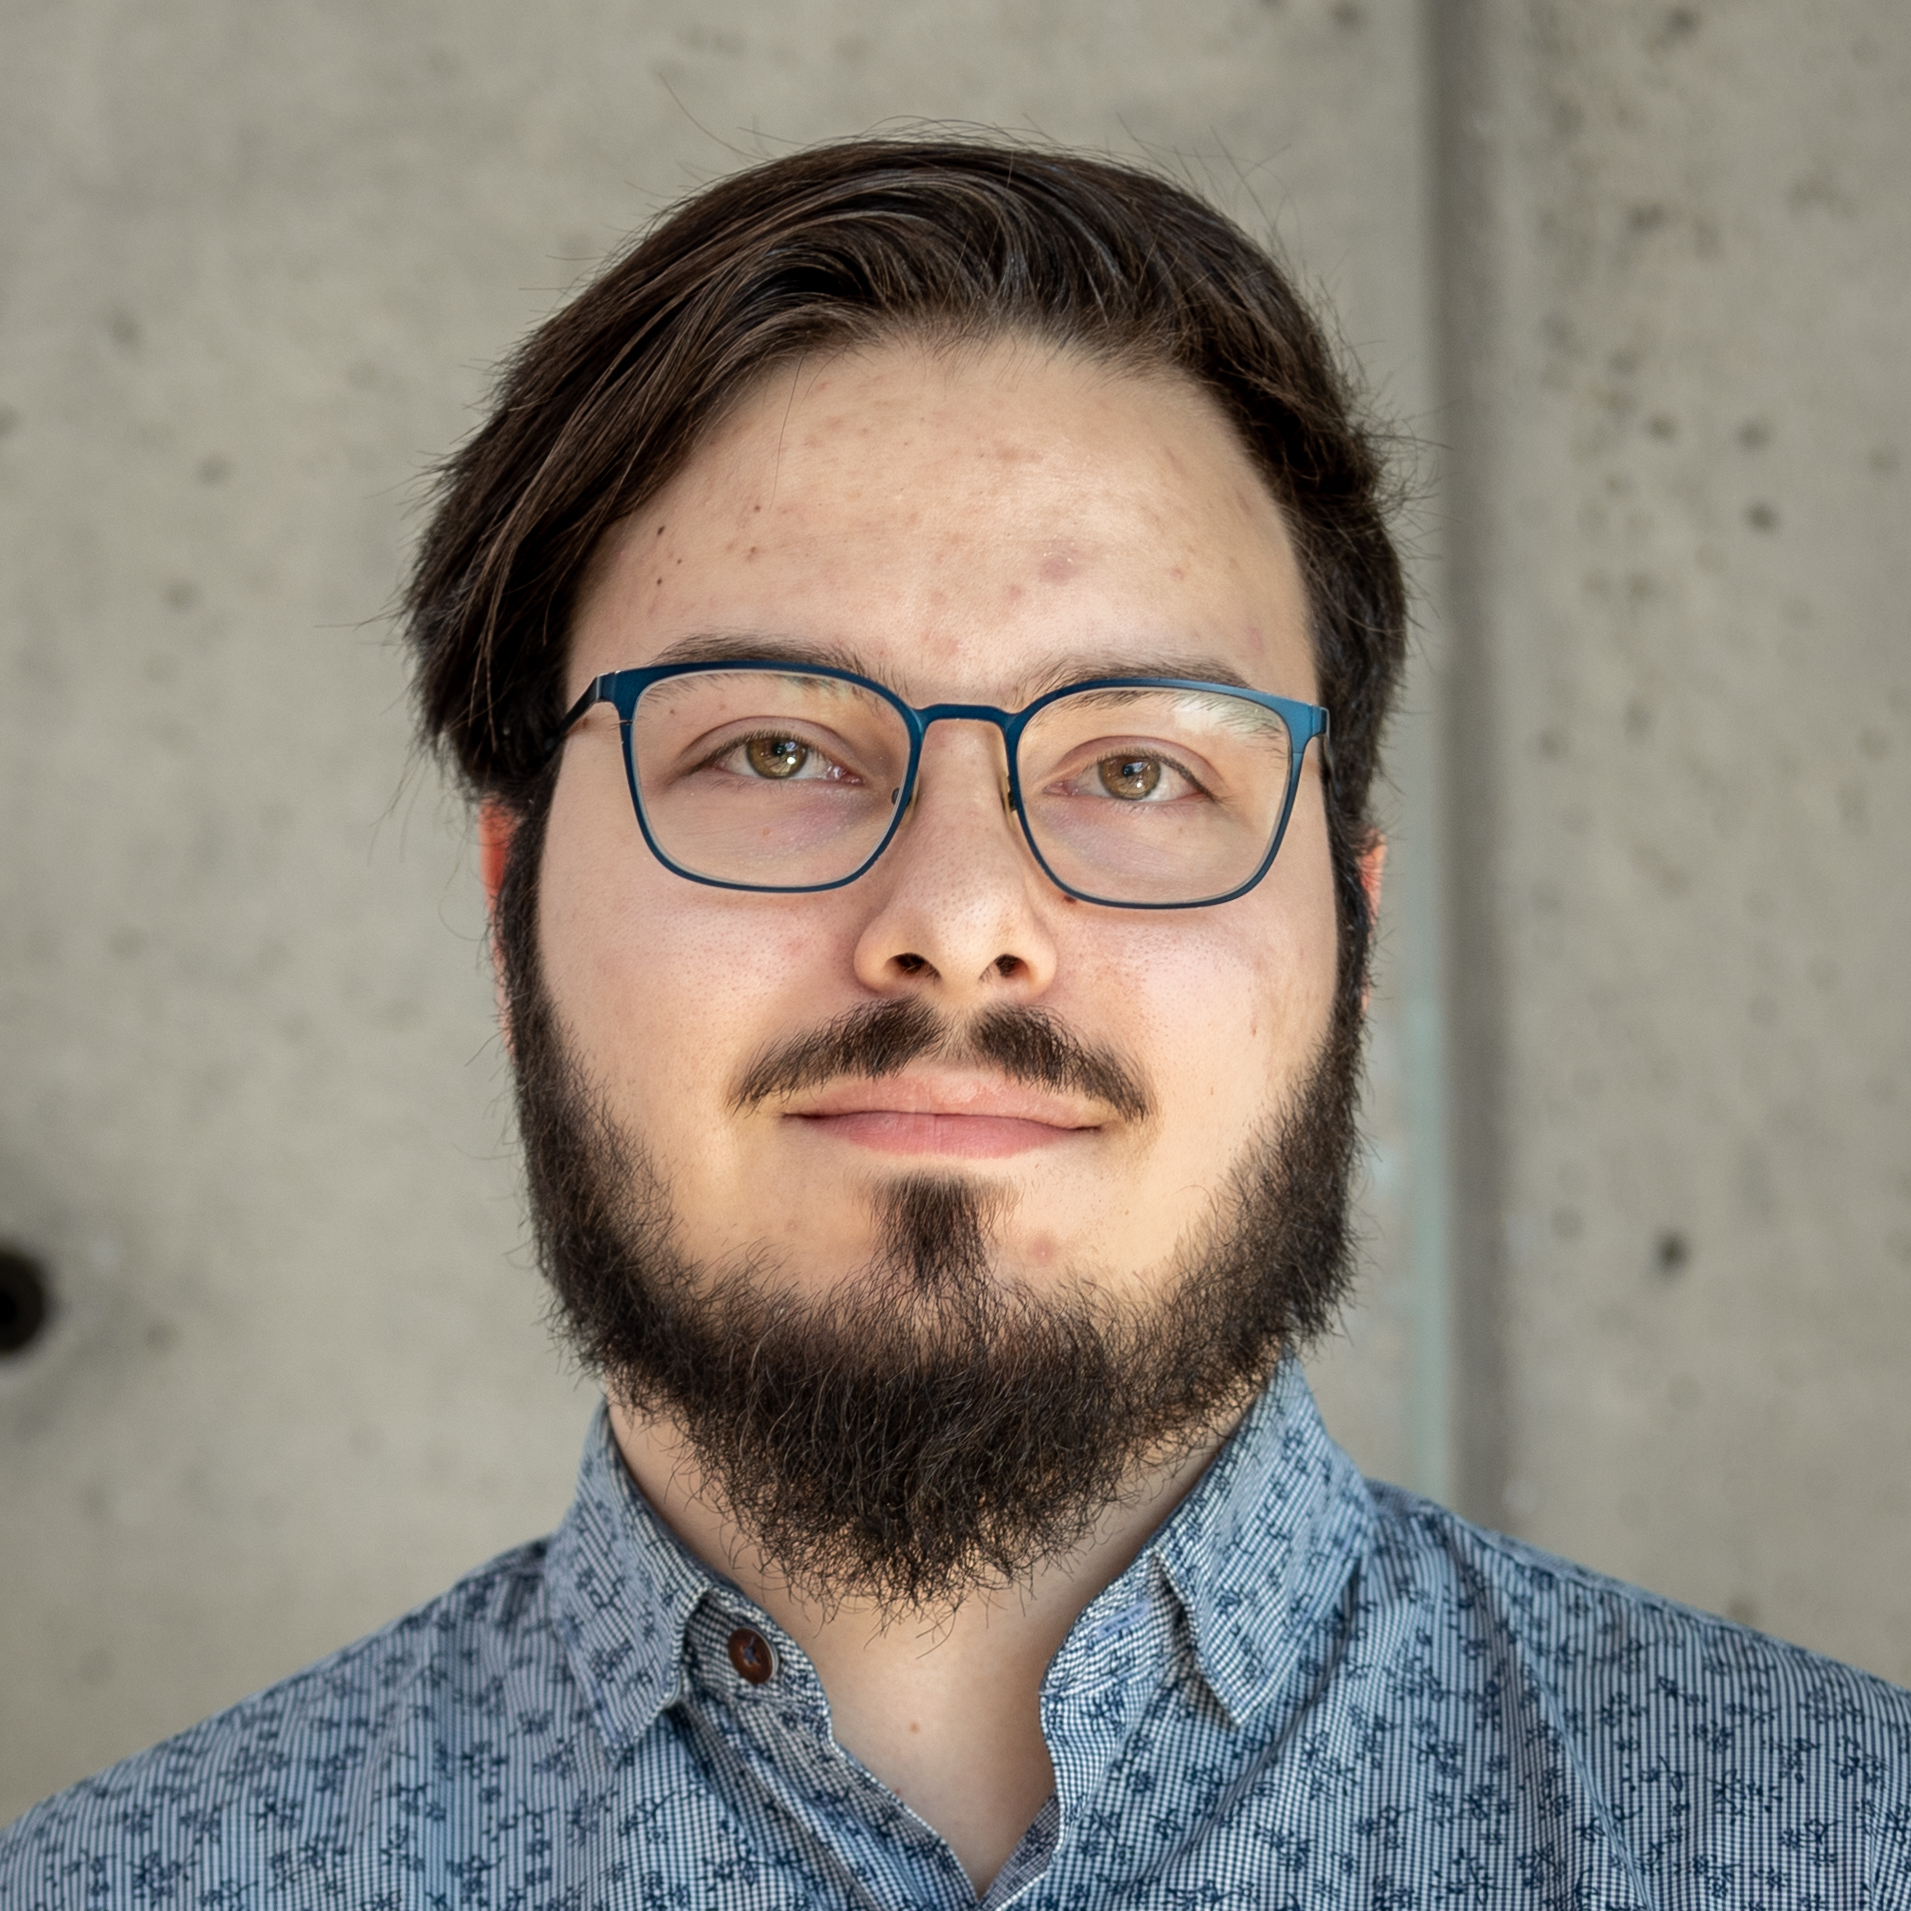
\includegraphics[width=0.9\linewidth]{img/membres/Charles-Ouzilleau-2.jpg} 
\end{wrapfigure}
\subsubsection*{}
\vspace{-2mm}
\textbf{Charles Ouzilleau}

Coque



\begin{wrapfigure}[5]{r}{0.25\textwidth}
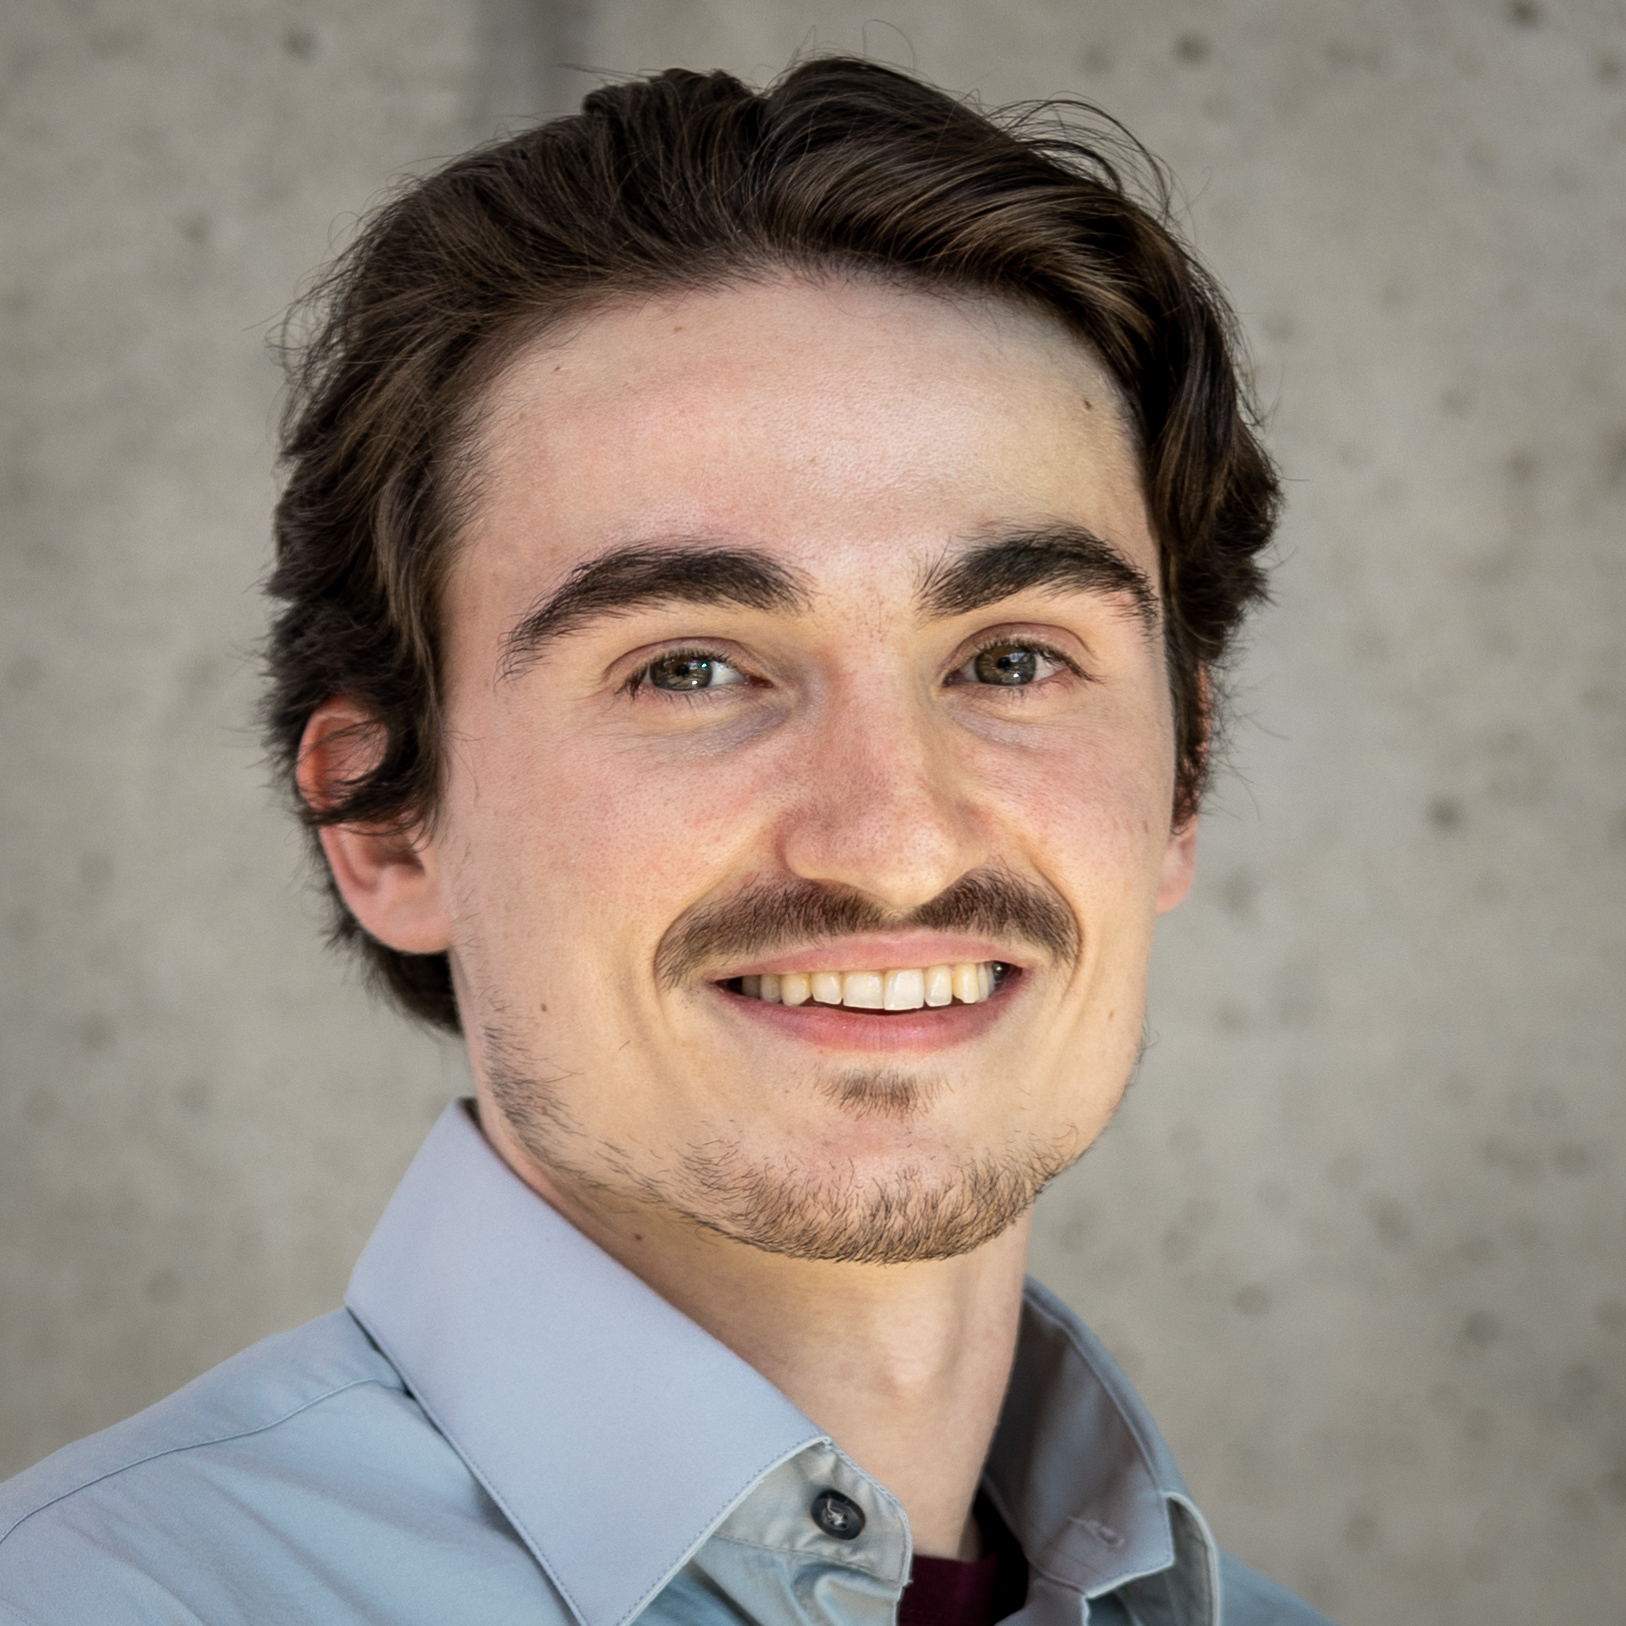
\includegraphics[width=.9\linewidth]{img/membres/Jean-Simon-D'Amours-Cyr-3.jpg} 
\end{wrapfigure}
\subsubsection*{}
\vspace{-2mm}
\textbf{Jean-Simon d'amours Cyr}

coque

Instrumentation


\begin{wrapfigure}[5]{r}{0.25\textwidth}
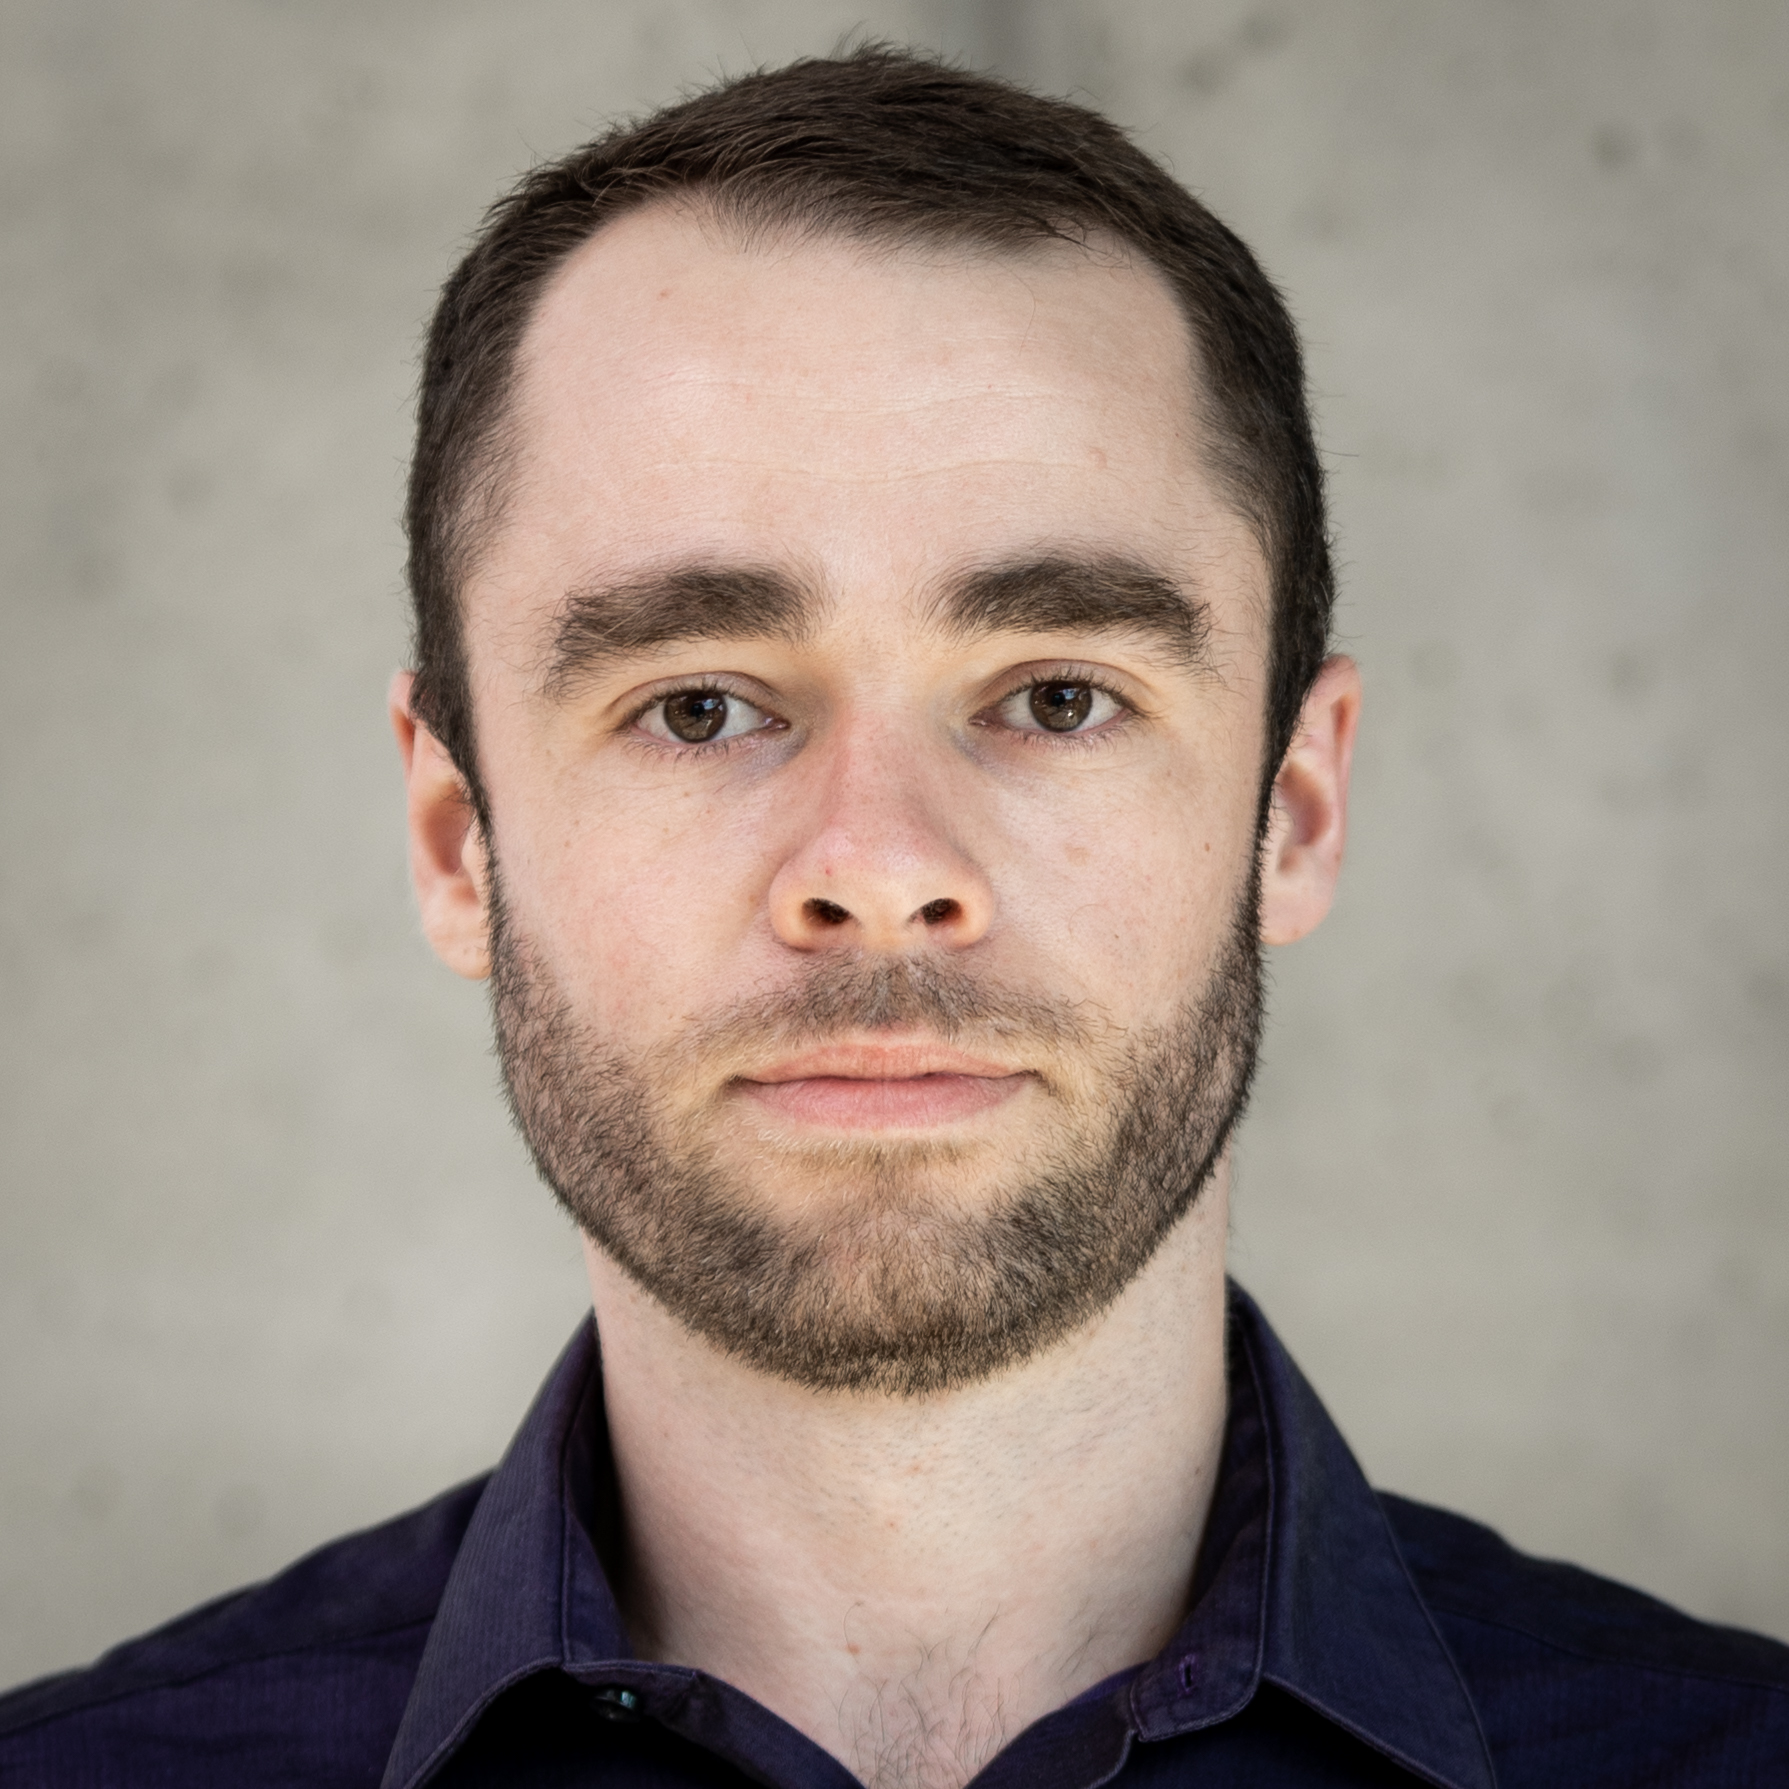
\includegraphics[width=.9\linewidth]{img/membres/Donald-Brouillard-2.jpg} 
\end{wrapfigure}
\subsubsection*{}
\vspace{2mm}
\textbf{Donald Brouillard}

Ch\^assis

\begin{wrapfigure}[5]{r}{0.25\textwidth}
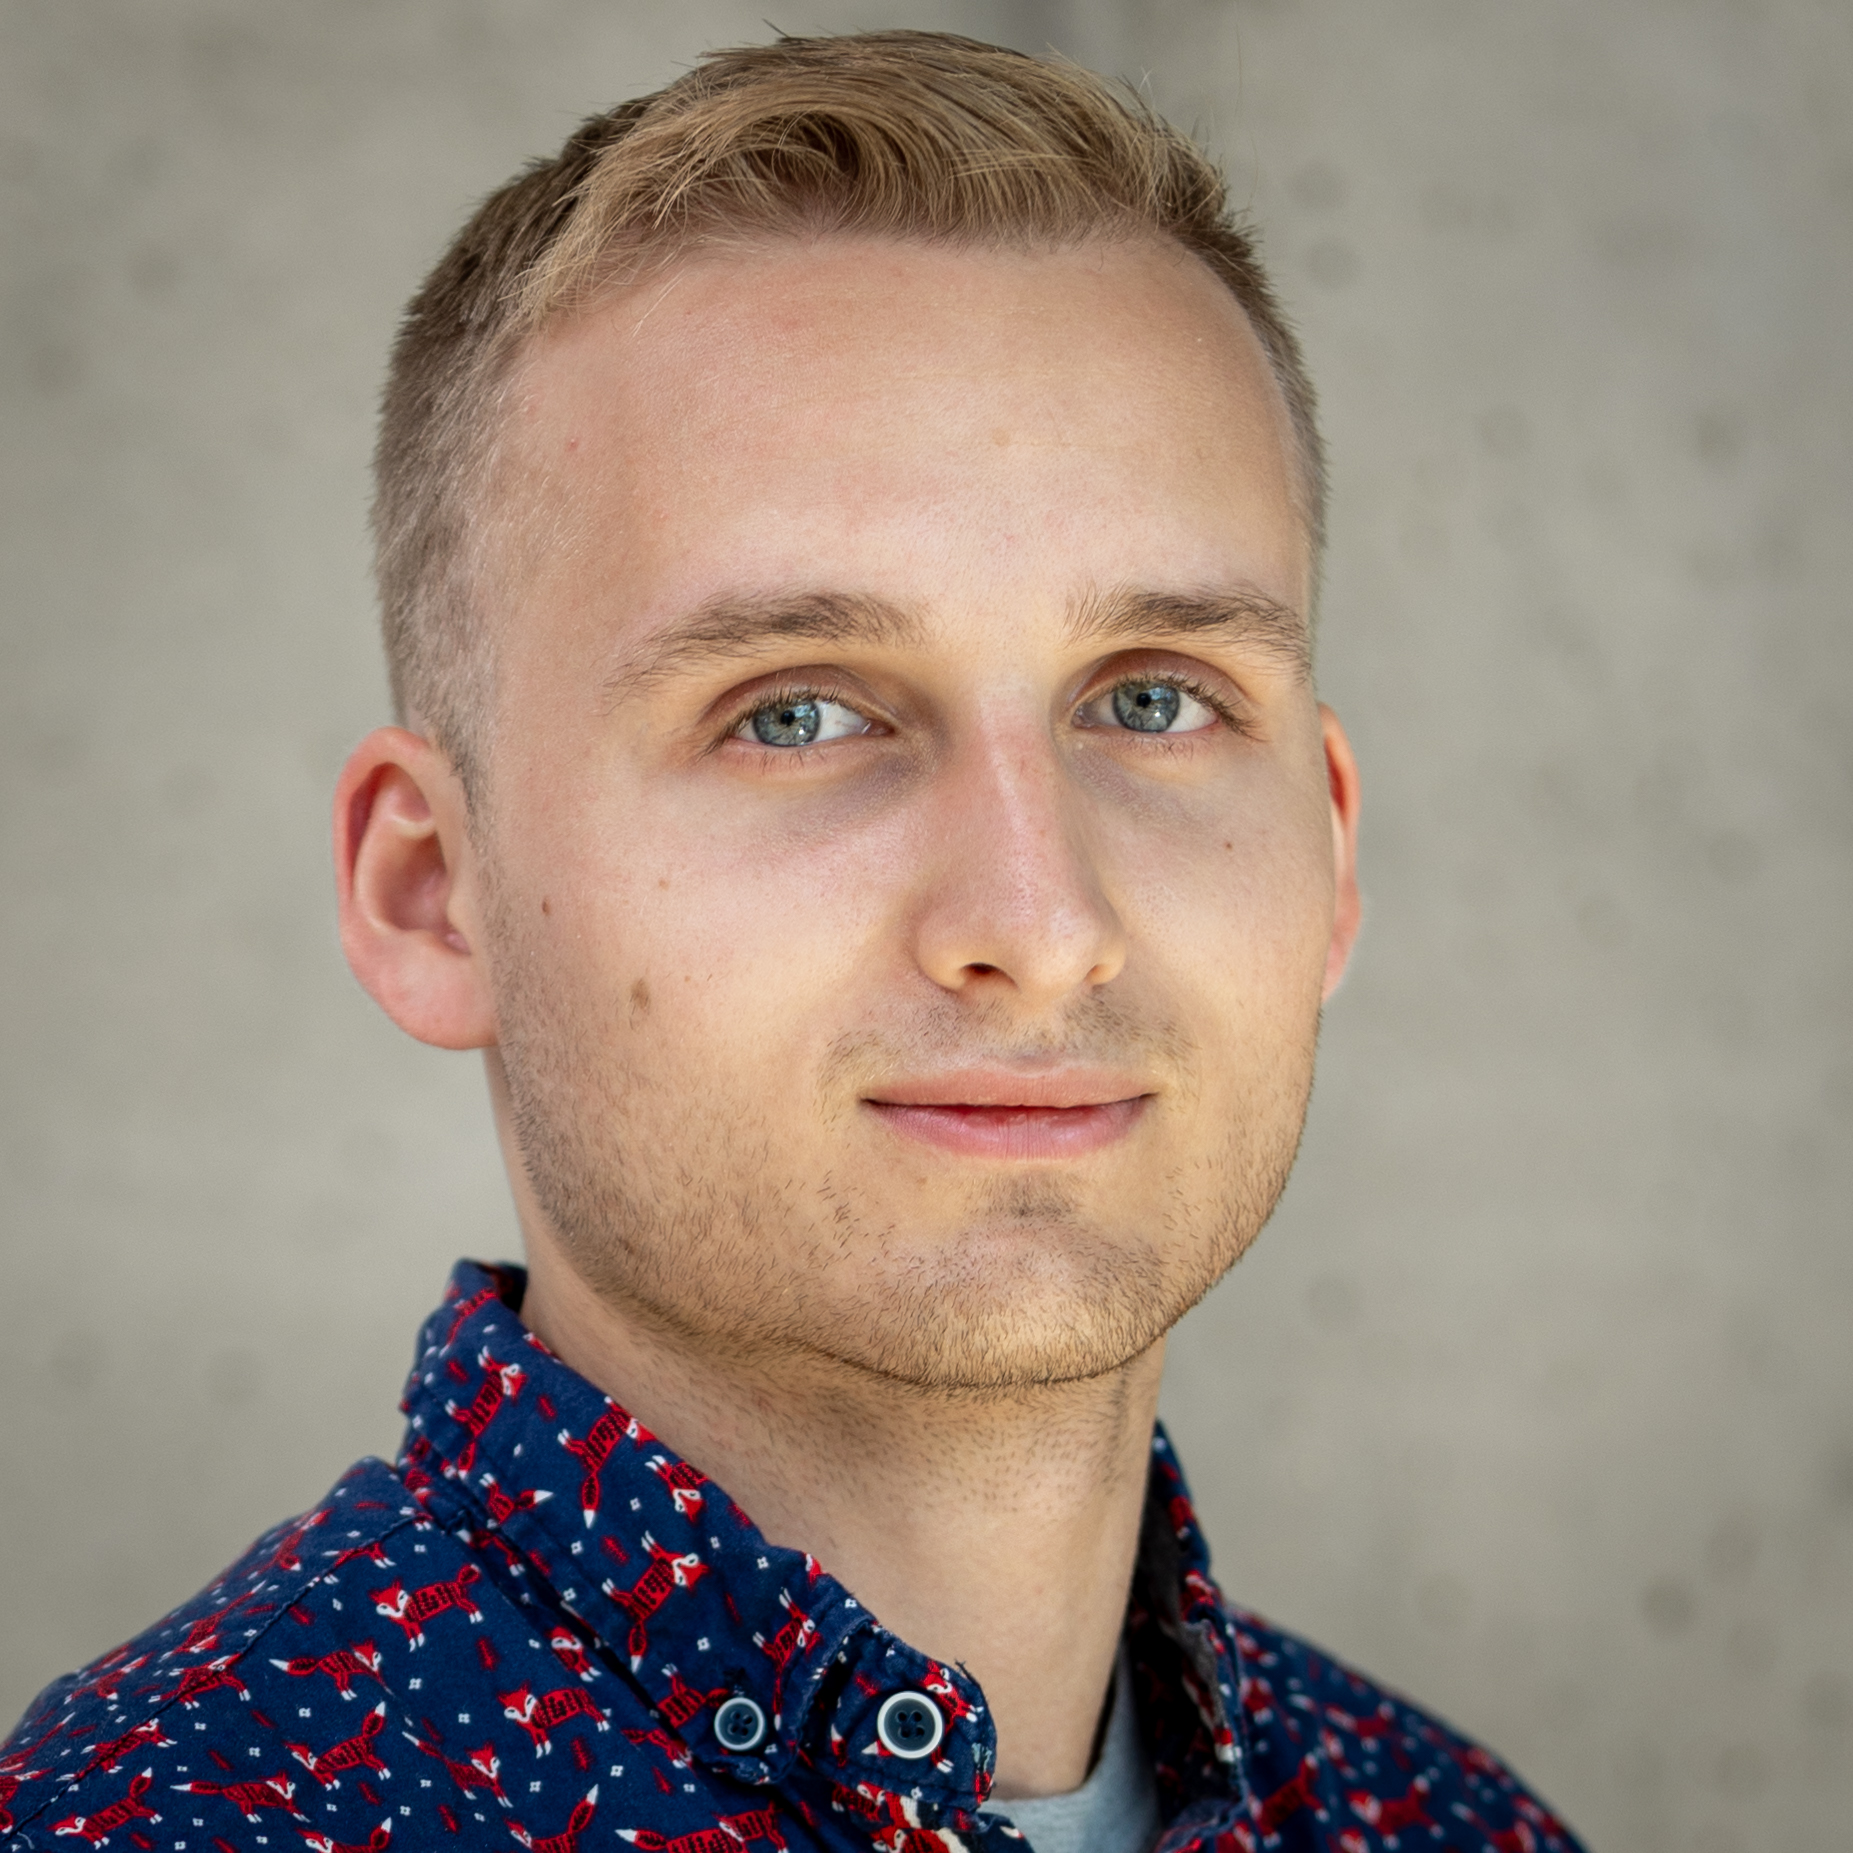
\includegraphics[width=.9\linewidth]{img/membres/Marco-Roger-3.jpg} 
\end{wrapfigure}
\subsubsection*{}
\vspace{2mm}
\textbf{Marco Roger}

Ch\^assis


\begin{wrapfigure}[5]{r}{0.25\textwidth}
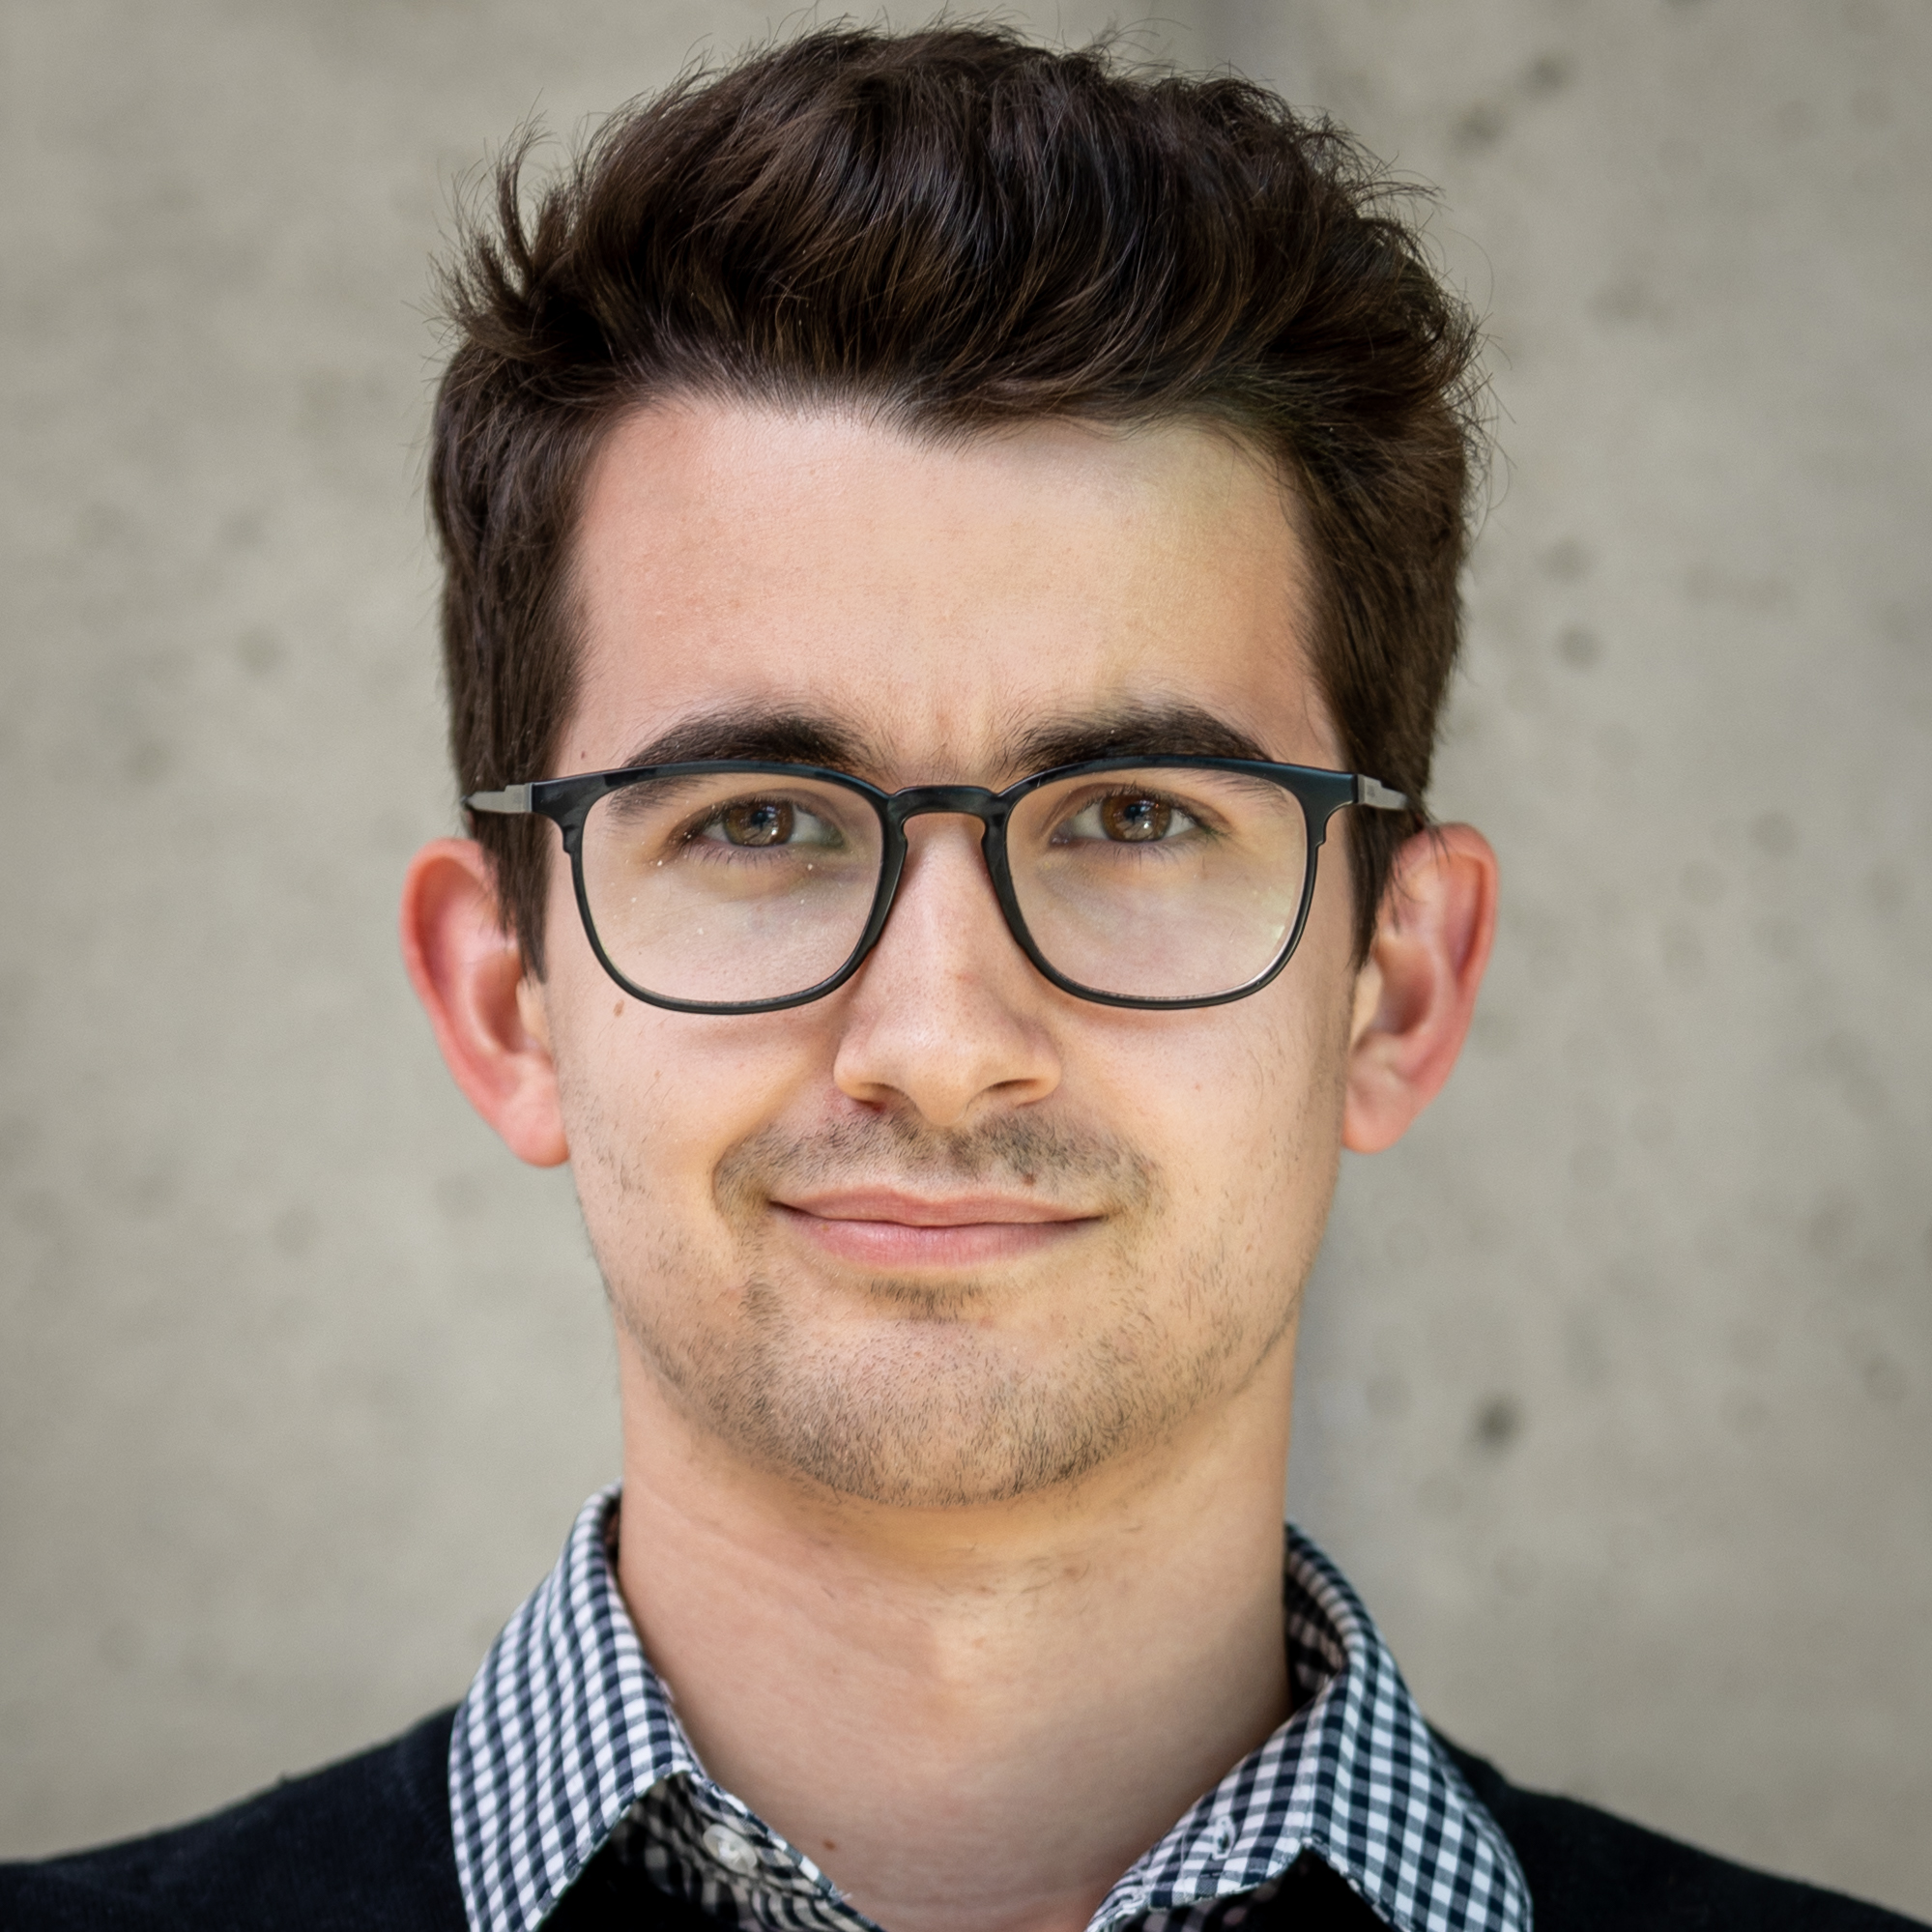
\includegraphics[width=.9\linewidth]{img/membres/Anthony-Martin-2.jpg} 
\end{wrapfigure}
\subsubsection*{}
\vspace{-2mm}
\textbf{Anthonny Martin}

Ch\^assis



\begin{wrapfigure}[5]{r}{0.25\textwidth}
\includegraphics[width=.9\linewidth]{img/membres/Joé-Morin-2.jpg} 
\end{wrapfigure}
\subsubsection*{}
\vspace{-2mm}
\textbf{Joé Morin}

Sous-syst\`eme (Ergo/CFD)



\begin{wrapfigure}[5]{r}{0.25\textwidth}
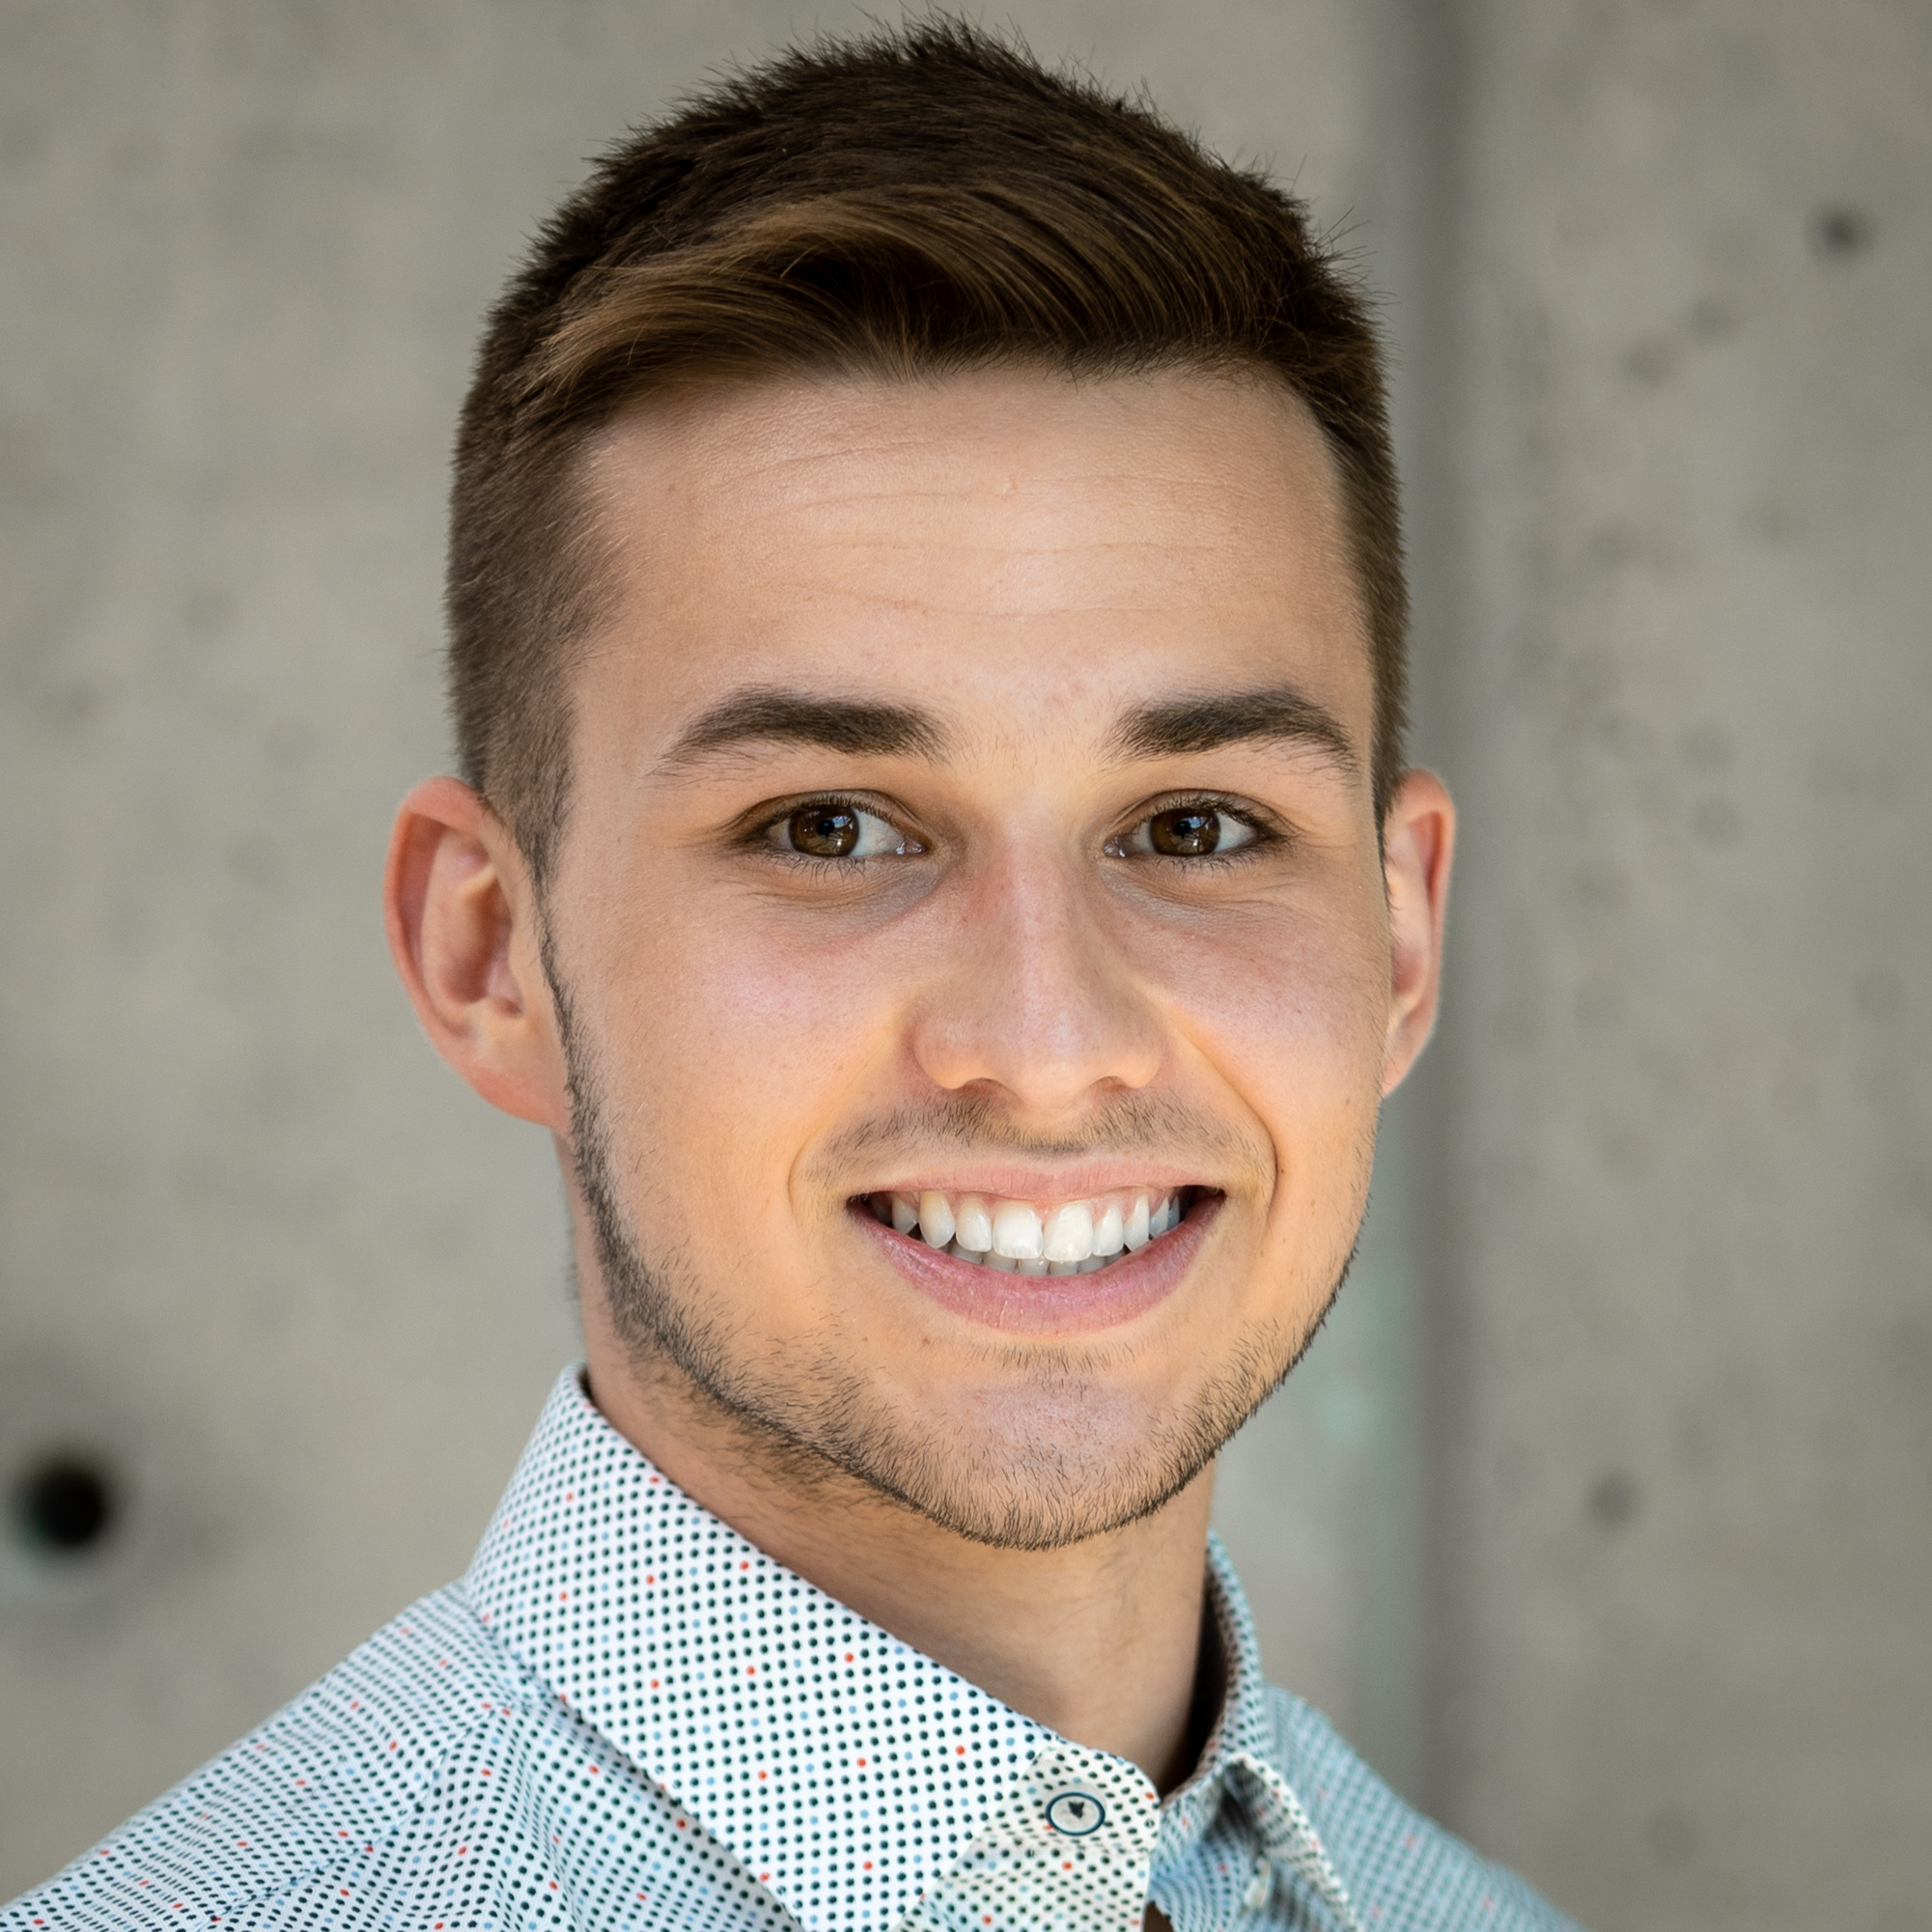
\includegraphics[width=.9\linewidth]{img/membres/Gabriel-Ouellet-3.jpg} 
\end{wrapfigure}
\subsubsection*{}
\vspace{2mm}
\textbf{Gabriel Ouellet}

Moteur / Transmission

\begin{wrapfigure}[5]{r}{0.25\textwidth}
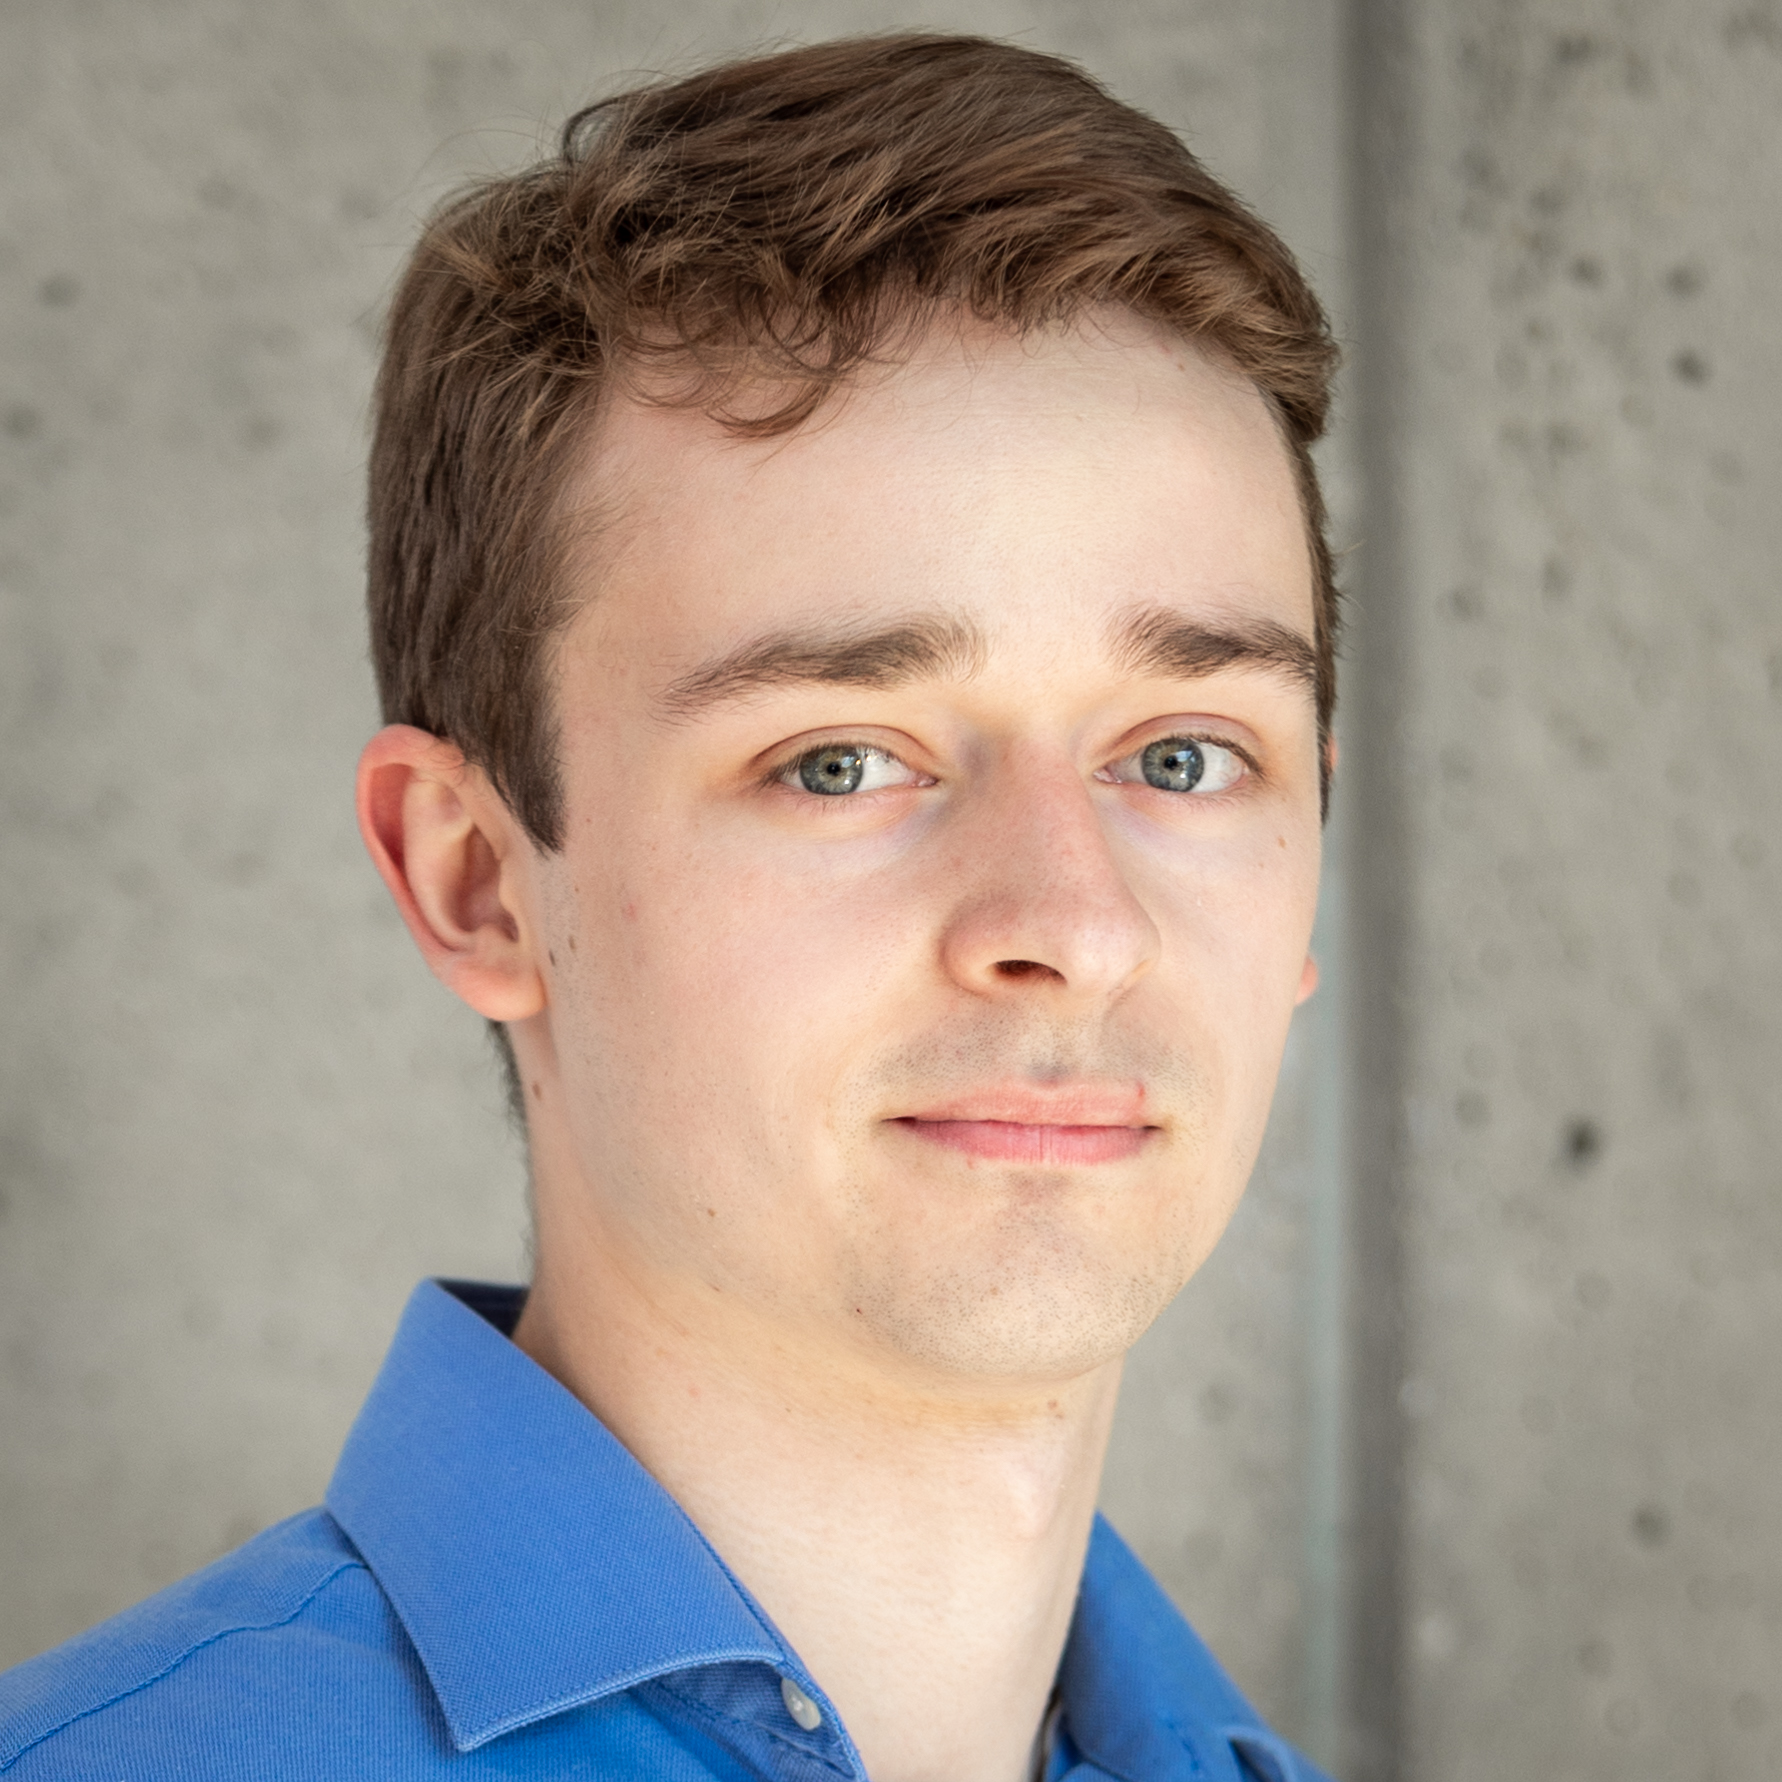
\includegraphics[width=.9\linewidth]{img/membres/Alexandre-Dumont-3.jpg} 
\end{wrapfigure}
\subsubsection*{}
\vspace{2mm}
\textbf{Alexandre Dumont}

Sous-syst\`eme (suspension/roue) et DT

\begin{wrapfigure}[5]{r}{0.25\textwidth}
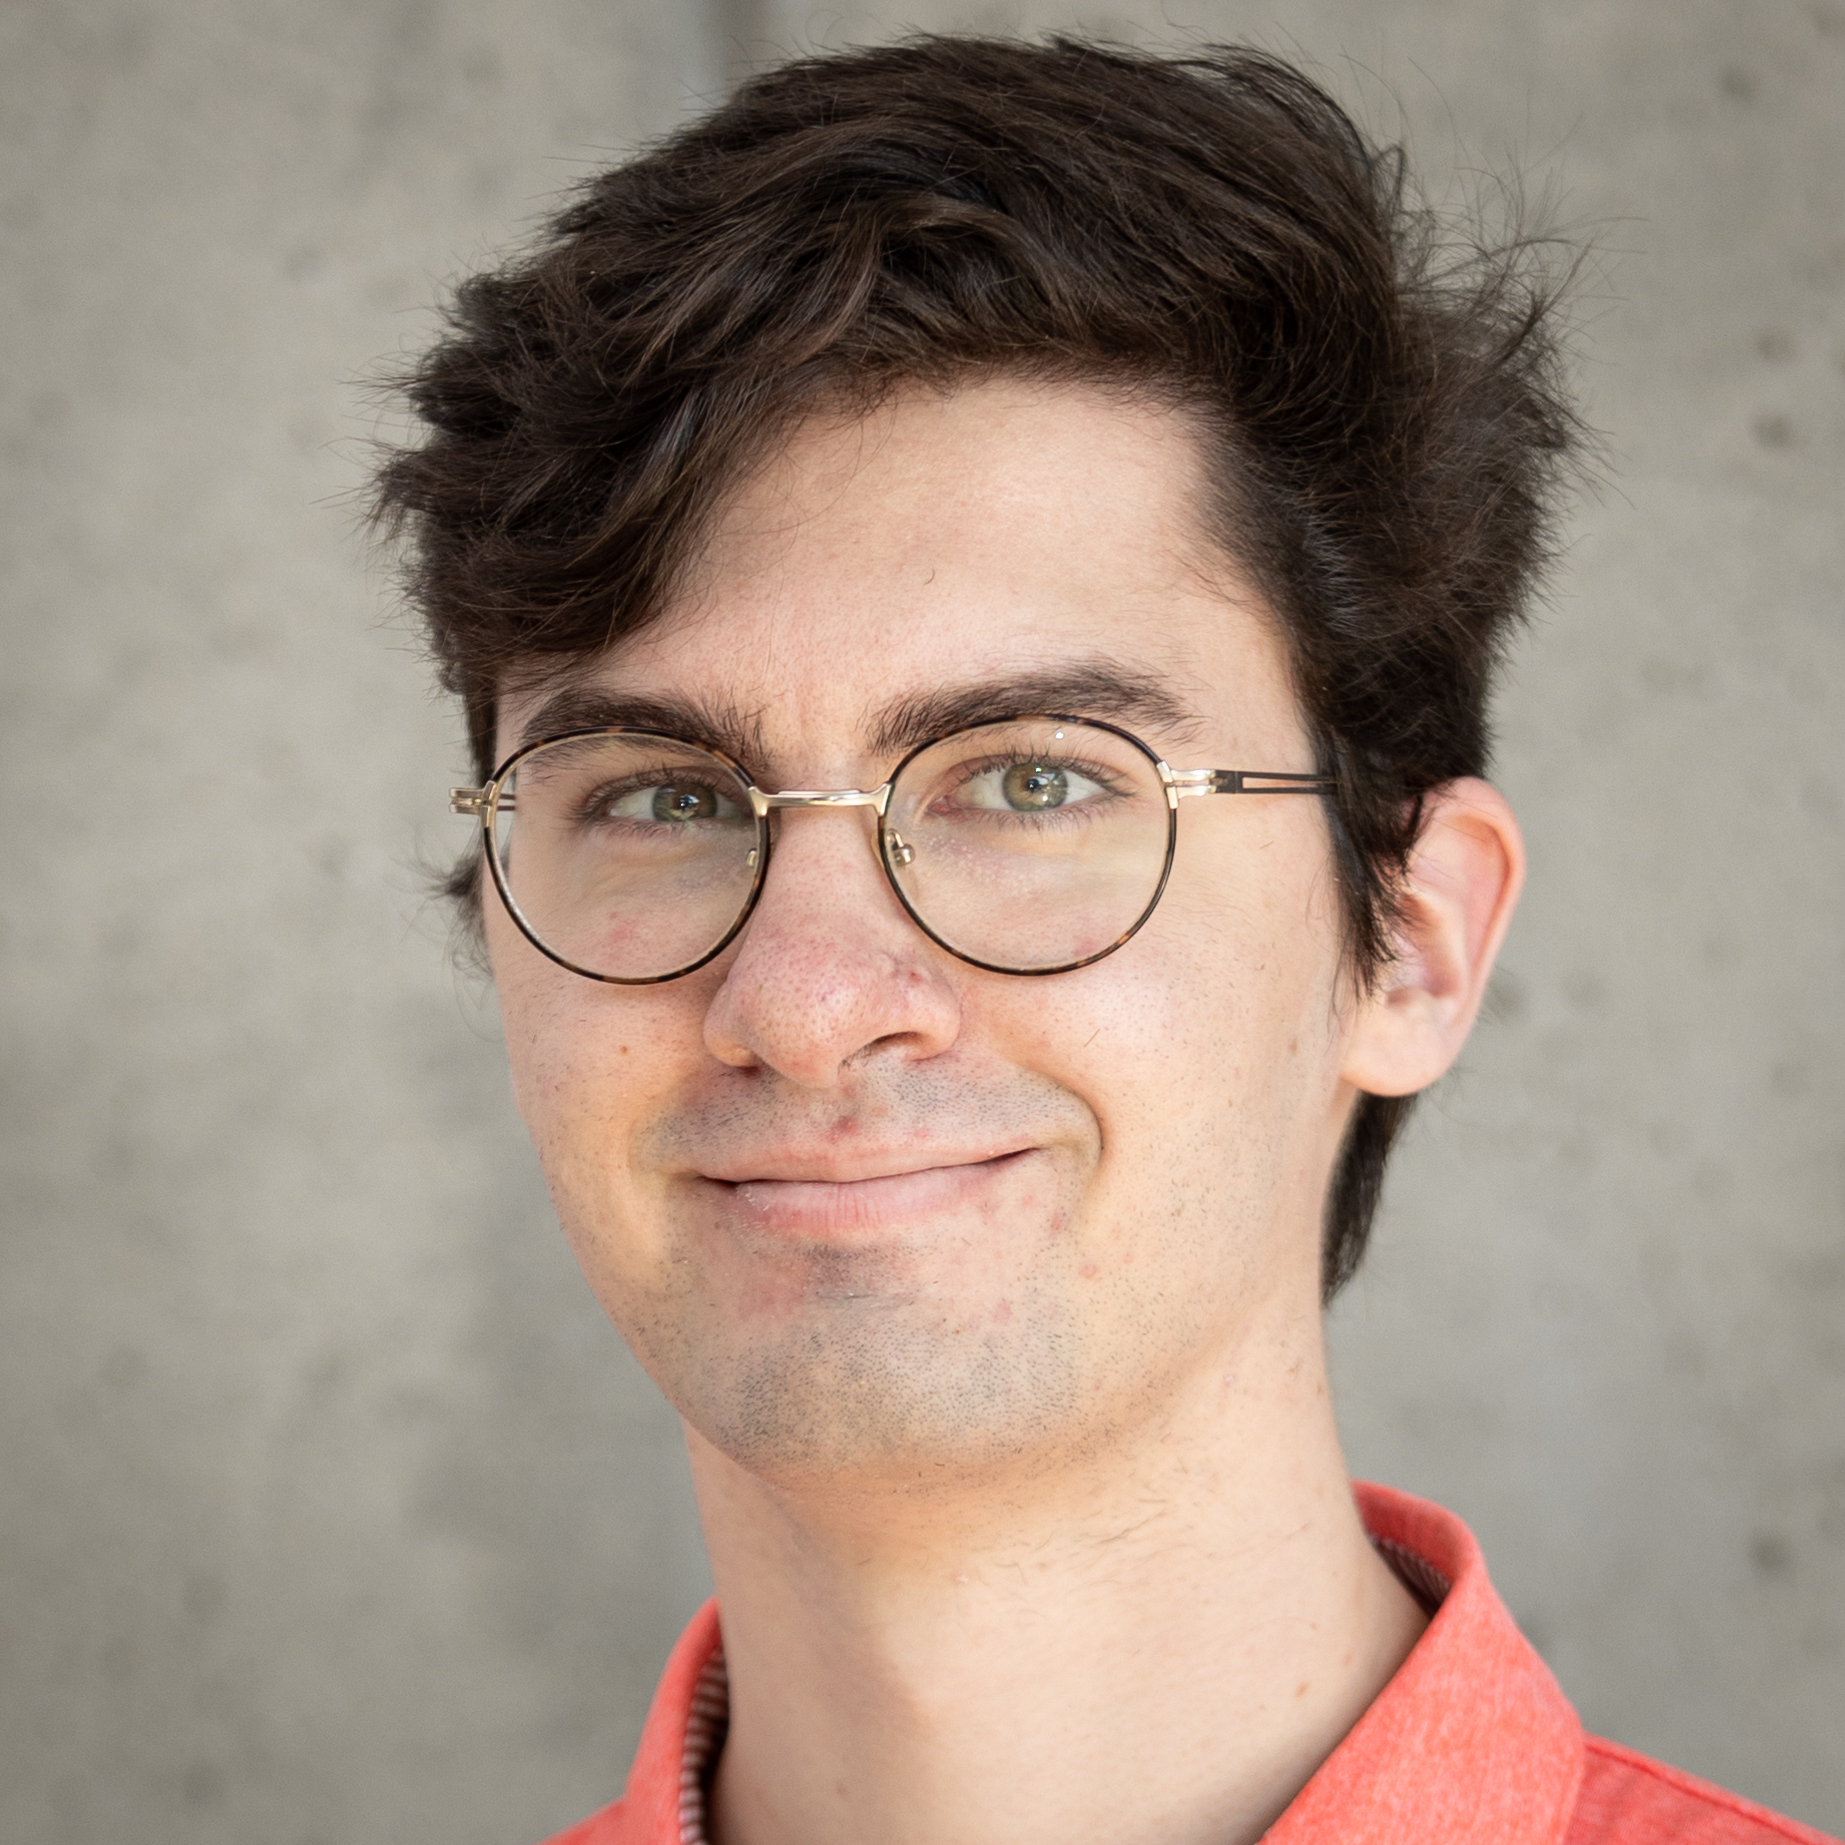
\includegraphics[width=.9\linewidth]{img/membres/Jérémi-Hamelin-3.jpg} 
\end{wrapfigure}
\subsubsection*{}
\vspace{2mm}
\textbf{Jérémi Hamelin}

Sous-syst\`eme (frein/suspension/roue)


\vspace{1cm}
%\begin{wrapfigure}[8]{r}{0.25\textwidth}
%\includegraphics[width=.9\linewidth]{DevOps.png} 
%\includegraphics[width=.9\linewidth]{DevOps.png} 
%\end{wrapfigure}
%
%\vspace{0.3cm}
%\subsubsection*{2. Another sub section:}
%
%Subsection description
%
%\vspace{2.3cm} %remove this, only added for spacing
%
%\begin{wrapfigure}[5]{r}{0.25\textwidth}
%\includegraphics[width=.9\linewidth]{TUDublin.jpg} 
%\end{wrapfigure}
%
%\vspace{0.35cm}
%\subsubsection*{3. Another sub section:}
%Final Subsection description
%
%\vspace{2cm} %remove this, only added for spacing
}


\headerbox{Courbe en S}{name=courbe_s,column=0,span=2,below=ordre_jour}{
{
    {
        \hspace{1cm}
        \centering
    	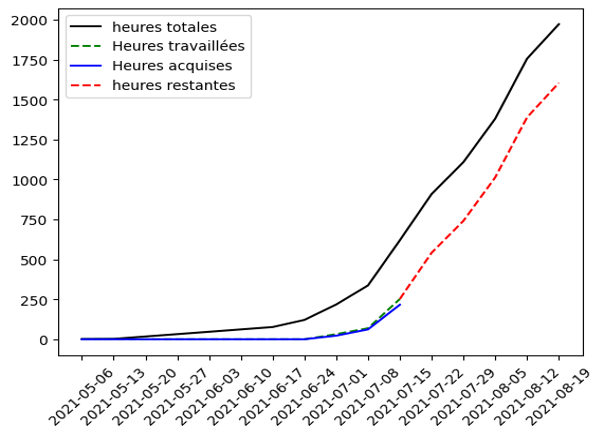
\includegraphics[scale=.54]{img/Courbe_S.png}
    }
}

}

\headerbox{Heures travaillées}{name=heures,column=0,span=2,below=courbe_s}{
{
    
    {
        \hspace{1cm}
        \centering
    	\includegraphics[scale=.75]{img/Heures_travaillees.png}
    }
    \vspace{1.3cm}
}

}

\end{poster}

\begin{poster}
{
grid=false,
headerborder=open, % Adds a border around the header of content boxes
colspacing=1em, % Column spacing
bgColorOne=white, % Background color for the gradient on the left side of the poster
bgColorTwo=white, % Background color for the gradient on the right side of the poster
borderColor=Mycolor1, % Border color
headerColorOne=Mycolor2, % Background color for the header in the content boxes (left side)
headerColorTwo=Mycolor2, % Background color for the header in the content boxes (right side)
headerFontColor=white, % Text color for the header text in the content boxes
boxColorOne=white, % Background color of the content boxes
textborder=rounded, %rectangle, % Format of the border around content boxes, can be: none, bars, coils, triangles, rectangle, rounded, roundedsmall, roundedright or faded
eyecatcher=false, % Set to false for ignoring the left logo in the title and move the title left
headerheight=0\textheight, % Height of the header
headershape=rounded, % Specify the rounded corner in the content box headers, can be: rectangle, small-rounded, roundedright, roundedleft or rounded
headershade=plain,
headerfont=\Large\textsf, % Large, bold and sans serif font in the headers of content boxes
%textfont={\setlength{\parindent}{1.5em}}, % Uncomment for paragraph indentation
linewidth=1pt % Width of the border lines around content boxes
}
{}
{\textsf{{}}} % Titre vide pcq sinon ça plante


% this states the box starts at column 0 (edge of page), row 0 (top of page) for a span of 3 (columns wide)
\headerbox{Tâches accomplies}{name=taches,column=0,row=0, span=3}{
{\textbf{\large Ch\^assis}\\\
\begin{tabularx}{\linewidth}{
    |>{\hsize=2.5\hsize}X|% 10% of 4\hsize 
    >{\hsize=0.5\hsize}X|% 30% of 4\hsize
    >{\hsize=0.5\hsize}X|% 30% of 4\hsize
    >{\hsize=0.5\hsize}X|% 30% of 4\hsize
       % sum=0.2\hsize for 4 columns
  }
    \hline
    \textbf{Objectif} & \textbf{Responsable} & \textbf{\% attendu} & \textbf{\% fait}
    \\\hline
        Conception et fabrication des Jigs pour découper les pièces du châssis & Marco & 100\% & 100\% \\\hline 
        Conception et fabrication des Jigs pour assembler le châssis & Marco & 100\% & 100\% \\\hline 
        Fabrication des panneaux de carbones chez Gurit & Donald & 100\% & 100\% \\\hline
        Laminage à la main du dessus des poutres & Donald & 100\% & 100\% \\\hline
        Ajout insert rond en fibre de carbone dans les poutres & Anthony & 100\% & 100\% \\\hline
        Assemblage du châssis & Anthony & 100\% & 100\% \\\hline 
        Fabrication de l'arceau (découpe, inserts, sablage, lamination) & Marco & 100\% & 100\%
        \\\hline 
        Intégration pentures de portes (jig,découpe, collage) & Anthony & 0\% & 0\%
        \\\hline
        Intégration direction (trous plancher et arseau) & Marco & 0\% & 0\%
        \\\hline
       
\end{tabularx}



\hfill \break
\textbf{\large Coque}\\
\begin{tabularx}{\linewidth}{
    |>{\hsize=2.5\hsize}X|% 10% of 4\hsize 
    >{\hsize=0.5\hsize}X|% 30% of 4\hsize
    >{\hsize=0.5\hsize}X|% 30% of 4\hsize
    >{\hsize=0.5\hsize}X|% 30% of 4\hsize
  }
    \hline
    \textbf{Objectif} & \textbf{Responsable}  & \textbf{\% attendu} & \textbf{\% fait} \\\hline
       Concept pour recouvrement du dessous des ailes avant & Charles & 80\% & 60\%
       \\\hline
       Conception des moules pour les ailes avant et arrière & Charles & 0\% & 0\%
       \\\hline
       Fabrication du moule du pare-brise (sablage + fibre de verre) & J-S & 90\% & 70\%
       \\\hline
       Fabrication des pare-chocs avant et arrière & J-S & 100\% & 75\%
       \\\hline 
       Renders et coloration pour coque - Amorcer les discussions & Joé & 15\% & 15\%
       \\\hline 
\end{tabularx}



\hfill \break
\textbf{\large Simulateur}\\
\begin{tabularx}{\linewidth}{
     |>{\hsize=2.5\hsize}X|% 10% of 4\hsize 
    >{\hsize=0.5\hsize}X|% 30% of 4\hsize
    >{\hsize=0.5\hsize}X|% 30% of 4\hsize
    >{\hsize=0.5\hsize}X|% 30% of 4\hsize
  }
    \hline
    \textbf{Objectif} & \textbf{Responsable}  & \textbf{\% attendu} & \textbf{\% fait} \\\hline
      Support à l'équipe informatique & Alex & NA& NA \\\hline 
\end{tabularx}



\hfill \break
\textbf{\large Suspension}\\
\begin{tabularx}{\linewidth}{
    |>{\hsize=2.5\hsize}X|% 10% of 4\hsize 
    >{\hsize=0.5\hsize}X|% 30% of 4\hsize
    >{\hsize=0.5\hsize}X|% 30% of 4\hsize
    >{\hsize=0.5\hsize}X|% 30% of 4\hsize
  }
    \hline
    \textbf{Objectif} & \textbf{Responsable}  & \textbf{\% attendu} & \textbf{\% fait} \\\hline


       Conception des nouveaux spacer &Alex & 100\% & 100\% \\\hline
       Fabrication des nouveaux spacer (Usinatech) &Alex & 100\% & 100\% \\\hline
       Soudure des arbres &Alex & 100\% & 100\% \\\hline
       Commande des anneaux 47 mm et des vis de freins&Alex & 100\% & 100\% \\\hline
       Modification des freins (interéfrence CAD)&Alex & 100\% & 100\% \\\hline
       Assemblage complet  &Alex & 100\% & 80\% \\\hline
       Intégration au châssis &Alex & 0\% & 0\% \\\hline
\end{tabularx}

\hfill \break
\textbf{\large Roues}\\
\begin{tabularx}{\linewidth}{
    |>{\hsize=2.5\hsize}X|% 10% of 4\hsize 
    >{\hsize=0.5\hsize}X|% 30% of 4\hsize
    >{\hsize=0.5\hsize}X|% 30% of 4\hsize
    >{\hsize=0.5\hsize}X|% 30% of 4\hsize
  }
    \hline
    \textbf{Objectif} & \textbf{Responsable}  & \textbf{\% attendu} & \textbf{\% fait} \\\hline
       Fabrication d'un nouveau moule pour la section centrale &Donald & 100\% & 100\% \\\hline  
       Fabrication des nouvelles sections centrales &Donald & 100\% & 100\% \\\hline  
       Assemblage des roues et installation des pneus &Donald & 75\% & 500\% \\\hline  

\end{tabularx}



\hfill \break
\textbf{\large Freins}\\
\begin{tabularx}{\linewidth}{
    |>{\hsize=2.5\hsize}X|% 10% of 4\hsize 
    >{\hsize=0.5\hsize}X|% 30% of 4\hsize
    >{\hsize=0.5\hsize}X|% 30% of 4\hsize
    >{\hsize=0.5\hsize}X|% 30% of 4\hsize
  }
    \hline
    Réception des pièces & Jérémi & 100\% & 90\% \\\hline
    Vérification interférence et frottement & Jérémi & 100\% & 80\% \\\hline
    Soudure des supports & Jérémi & 0\% & 0\% \\\hline
    Assemblage système complet et validations & Jérémi & 0\% & 0\% \\\hline
\end{tabularx}


\hfill \break
\textbf{\large Ergonomie}\\
\begin{tabularx}{\linewidth}{
    |>{\hsize=2.5\hsize}X|% 10% of 4\hsize 
    >{\hsize=0.5\hsize}X|% 30% of 4\hsize
    >{\hsize=0.5\hsize}X|% 30% of 4\hsize
    >{\hsize=0.5\hsize}X|% 30% of 4\hsize
  }
    \hline
    \textbf{Objectif} & \textbf{Responsable}  & \textbf{\% attendu} & \textbf{\% fait} \\\hline
 
       Fabrication du volant - intégration des composants (direction et instrumentation) & Joé & 90 \% &90\% \\\hline
       Fabrication essuie-glace - Impression 3D à faire & Joé & 20 \% & 20\% \\\hline
       Conception du support à lumières avant & Anthony & 80\% & 80\%
        \\\hline  
        Conception du support à lumières arrière & Anthony & 0\% & 0\%
        \\\hline 
        Fabrication des supports à lumières & Anthony & 0\% & 0\%
        \\\hline  
         Fabrication des pentures & Anthony & 50\% & 50\%
        \\\hline
         Fabrication couvercle bras de direction & Marco & 0\% & 0\%
        \\\hline
        Fabrication siège & Anthony & 0\% & 0\%
        \\\hline

\end{tabularx}

\hfill \break
\textbf{\large Direction}\\
\begin{tabularx}{\linewidth}{
    |>{\hsize=2.5\hsize}X|% 10% of 4\hsize 
    >{\hsize=0.5\hsize}X|% 30% of 4\hsize
    >{\hsize=0.5\hsize}X|% 30% of 4\hsize
    >{\hsize=0.5\hsize}X|% 30% of 4\hsize
  }
    \hline
    \textbf{Objectif} & \textbf{Responsable}  & \textbf{\% attendu} & \textbf{\% fait} \\\hline
        Élaborer un plan de validation des composantes & Gabriel  & 100\% & 60\%
        \\\hline
        Assembler le système de direction sur le véhicule & Gabriel & 0\% & 0\%


\end{tabularx}

\hfill \break
\textbf{\large Batterie}\\
\begin{tabularx}{\linewidth}{
    |>{\hsize=2.5\hsize}X|% 10% of 4\hsize 
    >{\hsize=0.5\hsize}X|% 30% of 4\hsize
    >{\hsize=0.5\hsize}X|% 30% of 4\hsize
    >{\hsize=0.5\hsize}X|% 30% of 4\hsize
  }
    \hline
    \textbf{Objectif} & \textbf{Responsable}  & \textbf{\% attendu} & \textbf{\% fait} \\\hline
        Conception de la boîte de protection du bloc-batterie & Jérémi & 90\% & 90\% \\\hline
\end{tabularx}

% --------------------------------------------------------------------------------
% Copy/Paste following code to add a new sub-system
% --------------------------------------------------------------------------------
% \hfill \break
% \textbf{\large SOUS_SYSTÈME}\\
% \begin{tabularx}{\linewidth}{
%     |>{\hsize=1.75\hsize}X|% 10% of 4\hsize 
%     >{\hsize=0.25\hsize}X|% 30% of 4\hsize
%       % sum=0.2\hsize for 4 columns
%   }
%     \hline
%     \textbf{Objectif} & \textbf{Responsable} \\\hline
%       & \\\hline 
%       & \\\hline
%       & \\\hline 
% \end{tabularx}}

%\vspace{2cm} %remove this, only added for spacing

}

% this states the box starts at column 0 (edge of page), directly below the box labelled subtopic1 for a span of 1 (column wide)

\headerbox{Problèmes}{name=problemes,column=0,below=taches,span=3}{

{\begin{tabularx}{\linewidth}{
    |>{\hsize=2.0\hsize}X|% 10% of 4\hsize 
    >{\hsize=0.5\hsize}X|% 30% of 4\hsize
    >{\hsize=0.5\hsize}X|% 30% of 4\hsize 
       % sum=0.2\hsize for 4 columns
  }
    \hline
    \textbf{Problème} & \textbf{Système} & \textbf{Responsable}
    \\\hline
    Démoulage difficile des roues en carbone & Suspension & Donald \\\hline
     %Problème & Système & Responsable \\\hline
  \end{tabularx}
    
    
 % Template des problèmes rencontrés:
 %
 % Problème : le problème rencontré cette semaine
 % Système  : le nom ou numéro système que le problème touche ex: Simulateur ou SIM1
 % Responsable : Nom ou Initiales du ou des personnes touchées par ce problèmes ex: G.C. C.E.G.
 %
 %  \hline
 %  \textbf{Problème} & \textbf{Système} & \textbf{Responsable}\\\hline
 %  Problème & Système & Responsable \\\hline
 %  Problème & Système & Responsable \\\hline
 %  Problème & Système & Responsable \\\hline
 %  Problème & Système & Responsable \\\hline
 %  Problème & Système & Responsable \\\hline
 %  Problème & Système & Responsable \\\hline
 %  Problème & Système & Responsable \\\hline
 %}

%\vspace{.65cm}
%\begin{itemize}
%    \item \textbf{Faire un schéma de dataflow du simulateur:} Mauvais compréhension du flow de données du %simulateur dans l'équipe informatique				
%    \item \textbf{Peux pas entrer les heures dans le DVP:} Courbe en S est pas représentative.	
%    \end{itemize}%

%    \vspace{1.8cm} % spacing vertical

}

% this states the box starts at column 0 (edge of page), directly below the box labelled introduction for a span of 1 (column wide)
\headerbox{Avancement systèmes}{name=systemes,column=0,below=problemes,span=3}{

%\vspace{0.15cm}
\centering
{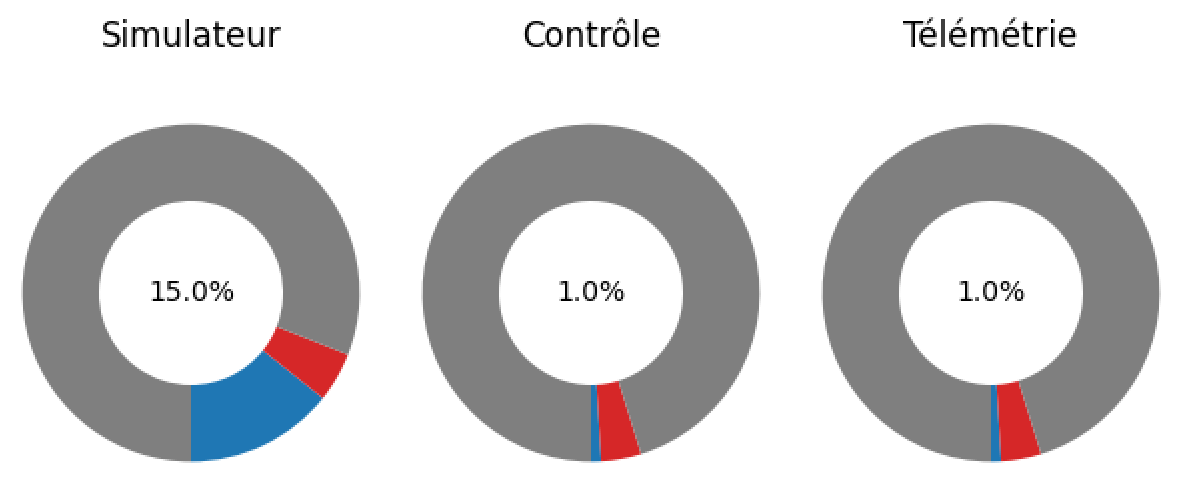
\includegraphics[width=1\linewidth]{img/avancement.png}}

%\vspace{0.2cm} % spacing vertical

}



\headerbox{Risques}{name=risques,column=0,span=3,below=systemes}{
{
    {\begin{tabularx}{\linewidth}{
    |>{\hsize=0.40\hsize}X|% 10% of 4\hsize 
    >{\hsize=0.25\hsize}X|% 30% of 4\hsize
    >{\hsize=0.25\hsize}X|% 30% of 4\hsize 
    >{\hsize=0.1\hsize}X|% 30% of 4\hsize 
       % sum=0.2\hsize for 4 columns
  }
    \hline
    \textbf{Risque} & \textbf{Mitigation} & \textbf{Conséquence} & \textbf{Priorité}\\\hline
    Usinage de pièces.&Commandite, ou valider avec BRP.&Pouvoir faire usiner les pièces rapidement & 4/5\\\hline
     Temps accorder au projet - Remises et Examens.&--.& Prévoire une diminution des heures dans RISE.(Moments pour rattraper?)  & 2/5
     &  &  &     
  \end{tabularx}
  
  
% Template pour le tableau des risques de la semaine : 

% Risque : le risque de la semaine
% Mitigation: comment mitiger le risque pour réduire ses conséquences/occurances/etc.
% Conséquence : La ou les conséquences si le risque survient
% Priorité : Priorité du risque sur une échelle de 1 à 5.  5 étant + prioritaire. La priorité est basé sur les conséquences la probablité d'occurence, etc.  
  
%  \textbf{Risque} & \textbf{Mitigation} & \textbf{Conséquence} & \textbf{Priorité}\\\hline
%    Risque & Mitigation & Conséquence & Priorité\\\hline
%    Risque & Mitigation & Conséquence & Priorité\\\hline
%    Risque & Mitigation & Conséquence & Priorité\\\hline
%    Risque & Mitigation & Conséquence & Priorité\\\hline
%    Risque & Mitigation & Conséquence & Priorité\\\hline
%    Risque & Mitigation & Conséquence & Priorité\\\hline
%    Risque & Mitigation & Conséquence & Priorité\\\hline
%    Risque & Mitigation & Conséquence & Priorité\\\hline
%    Risque & Mitigation & Conséquence & Priorité\\\hline
%    Risque & Mitigation & Conséquence & Priorité\\\hline
%    Risque & Mitigation & Conséquence & Priorité\\\hline
%    Risque & Mitigation & Conséquence & Priorité\\\hline}
}

}

\headerbox{Objectifs semaine prochaine}{name=objectifs_prochain,column=2,span=1,below=risques}{
{
    \vspace{.65cm}
    \begin{itemize}
    \item \textbf{Simulateur :}
    \begin{enumerate}
        \item 
        \item 
    \end{enumerate}
    \item \textbf{Coque :}
    \begin{enumerate}
        \item Réaliser 2 à 3 simulation complètes et fournir des pistes d'améliorations pour les itérations subséquentes
    \end{enumerate}
    \item \textbf{Direction/Suspension/freins :}
    \begin{enumerate}
        \item mettre ensemble les assemblages		
    \end{enumerate}
    \item \textbf{Gestion et Documentation :}
    \begin{enumerate}
        \item Séparer les parties du RCP1
        \item 	
    \end{enumerate}
    \end{itemize}
    
    \vspace{1cm} % spacing vertical
}

}

\headerbox{Cashflow}{name=cashflow,column=0,span=2,below=risques}{
{

    \vspace{.6cm} % spacing vertical
    {
        \hspace{1cm}
        \centering
    	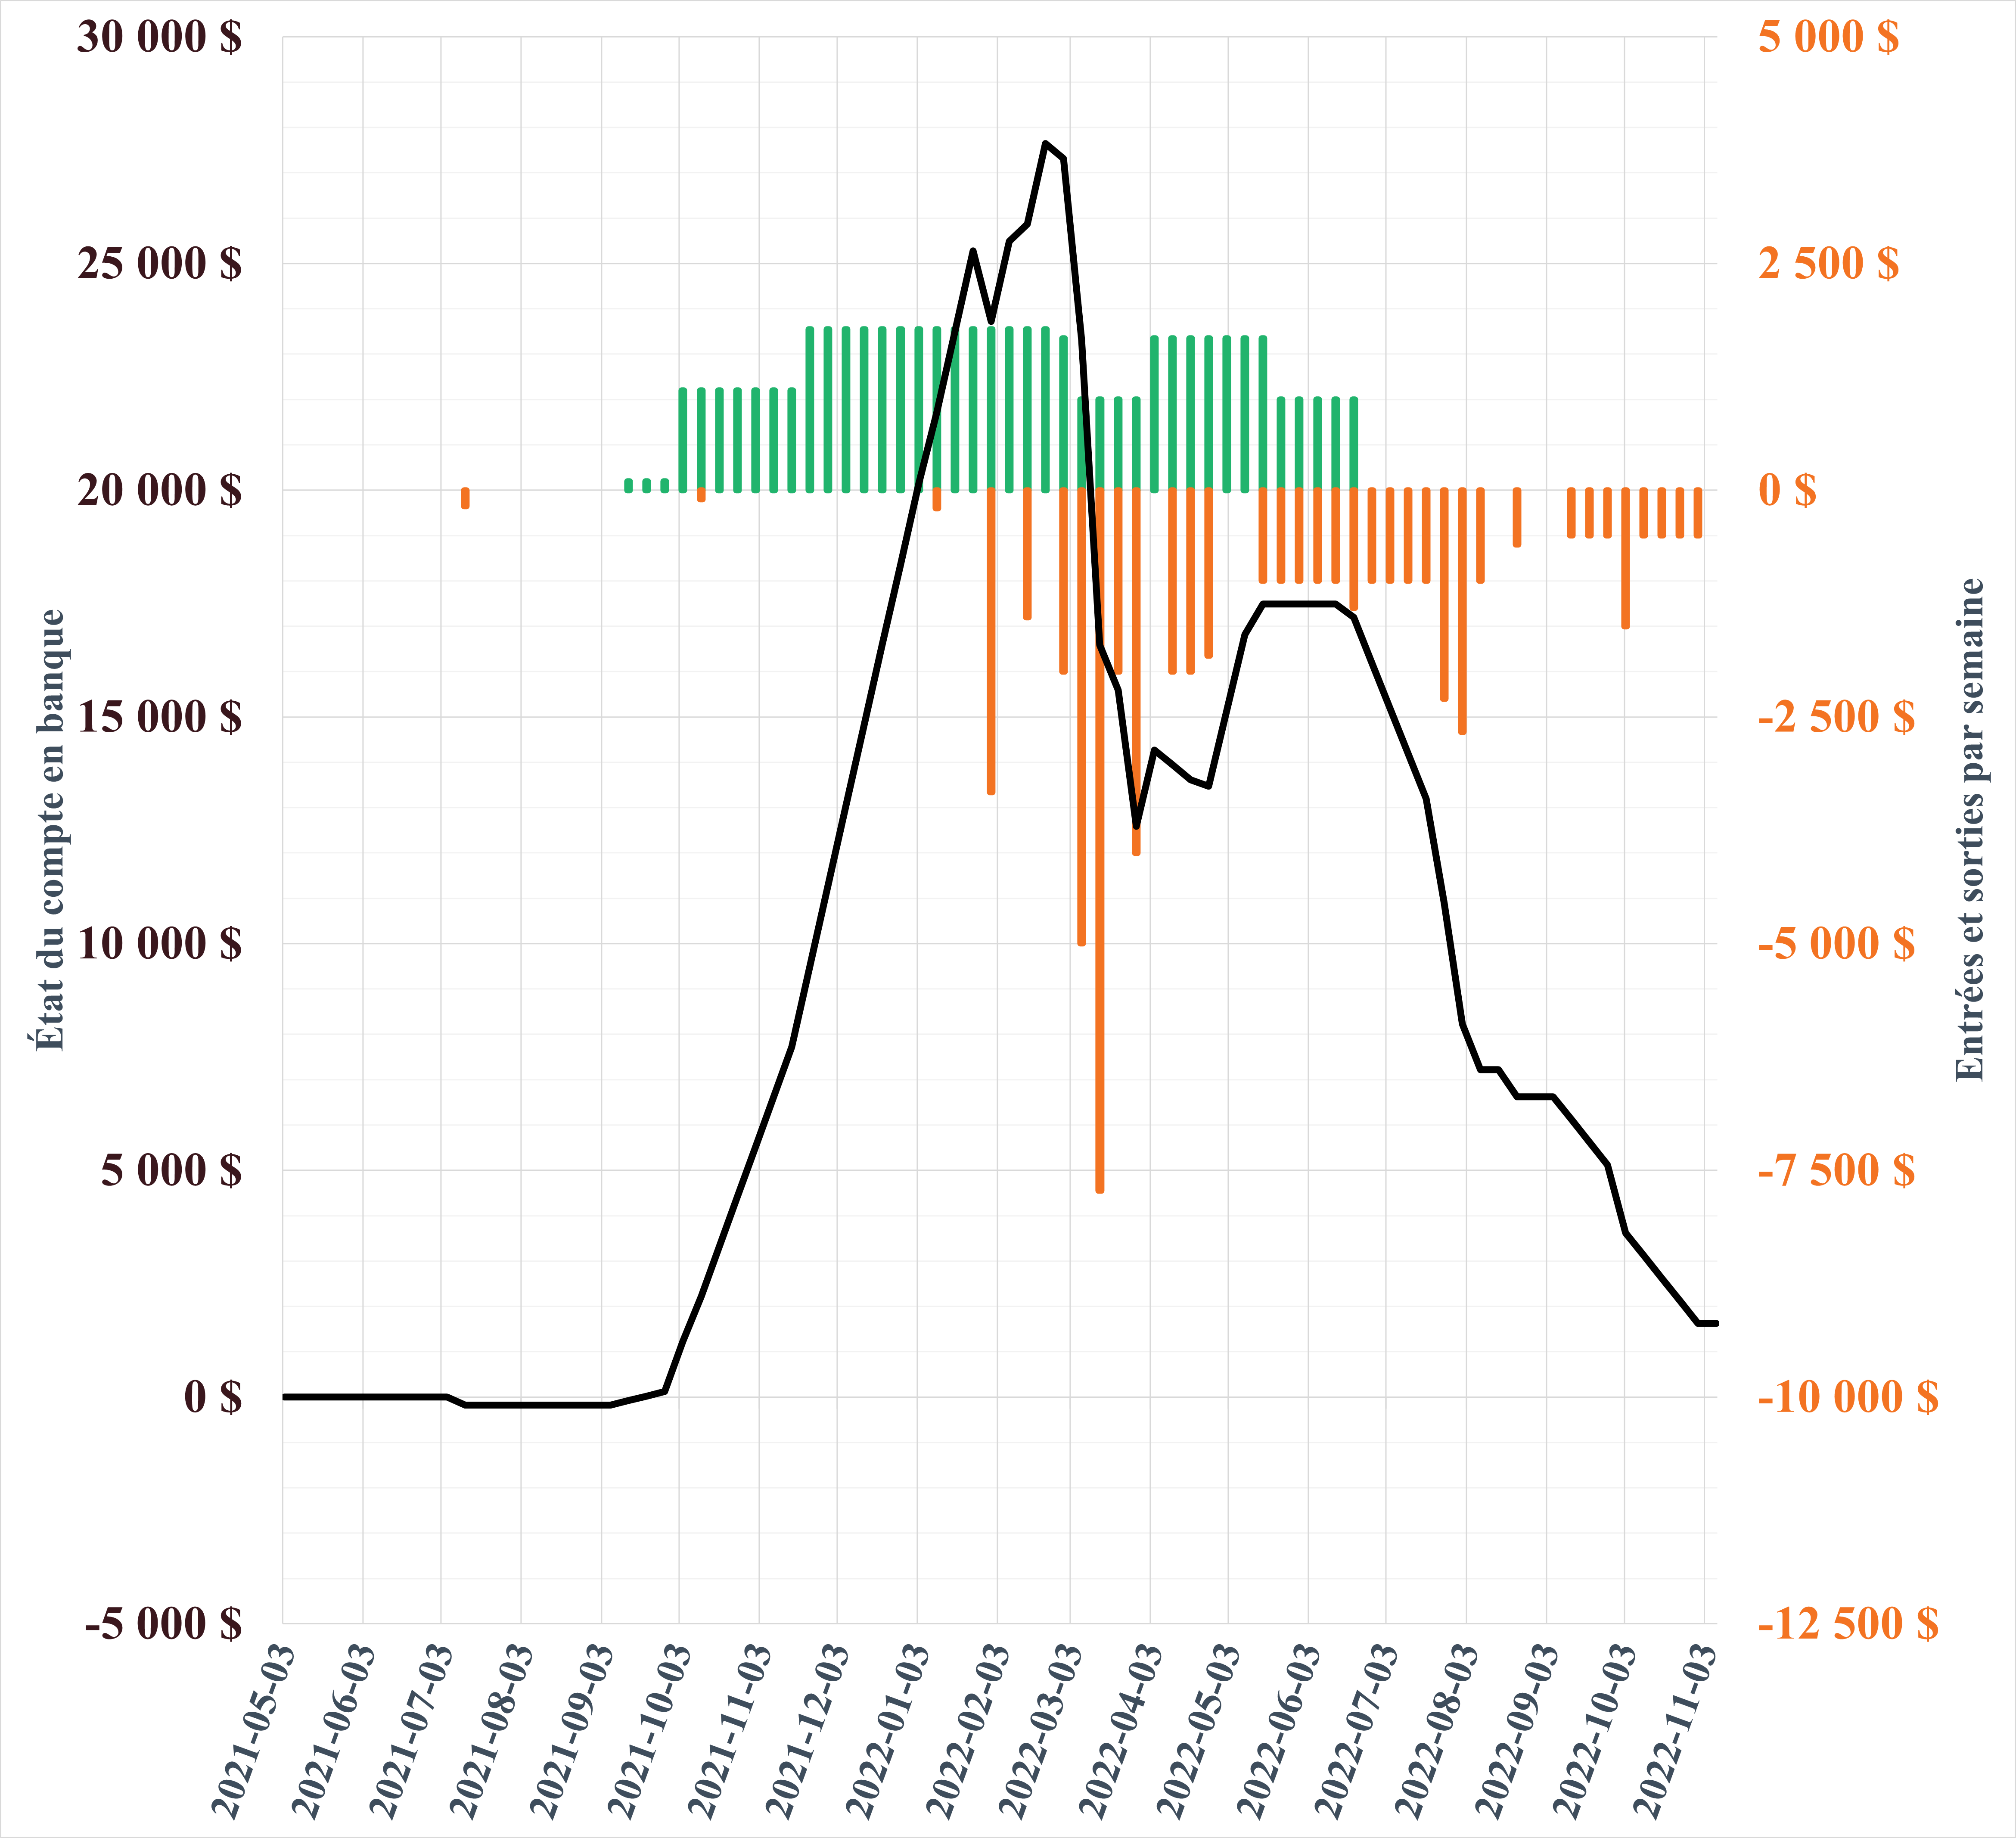
\includegraphics[scale=.5]{img/cashflow.png}
    }
    %\vspace{1.15cm} % spacing vertical
}

}

\end{poster}




\end{document}
